% Autor: Lukas Deeken
% Letzte Bearbeitung: 01.05.2022

\chapter{Elektromechanische Systeme}

\section{Akkumulator}
An dieser Stelle geht mein Dank an Tim Schweers, der dieses Projekt besonders in der mechanischen Auslegung und der Konstruktion so tatkräftig mitgetragen hat.

\subsection{Die Akkuzelle}

Wichtig bei der Zellenauswahl ist das stets jede individuelle Zelle für sich begutachtet werden muss. Es gibt bei den diversen Bauformen und chemischen Zusammensetzungen gewissen Tendenzen welche im Folgenden erläutert werden. Jedoch ist die Überlappung dieser Eigenschaften in der Regel so groß das sich augenscheinlich vollkommen unterschiedliche Zellen für einen ähnlichen Einsatzzweck eignen.
\FloatBarrier
\subsubsection{Vergleich der Speicherarten}

Im nachfolgenden wird die zuerst die Energie berechnet die ein Formula Student Fahrzeug bei einem Bremsvorgang freisetzt und damit die Energie die man speichern können müsste um mit der Speicherform auf sinnvolle Art und Weise eine Rekuperation umzusetzen. Im Anschluss wird diese Energie in eine ungefähre Masse umgesetzt um zu zeigen inwiefern sich diese Form der Energiespeicherung für den Einsatz eignet. Im nachfolgenden wird die Masse bestimmt um 6 KWh Energie zu speichern da, dies der Energieverbrauch eines Formula Student Fahrzeuges in der Disziplin des Endurance ist. Dieser Wert wurde im Rahmen eines Benchmarkings mit den Fahrzeugen anderer Teams über die letzten Jahre 2016 bis 2019, sowie einer \acfirst{LTS} errechnet.
\\
\\
Im folgenden errechnen wir die Energie welche bei einem durchschnittlich Bremsvorgang eines Formula Student Fahrzeug aufgenommen werden müsste. 

\begin{equation}
\glsc{symb:E_kin} = \dfrac{1}{2} * \glsc{symb:m} * \glsc{symb:v}^2
\end{equation}

\begin{table}[h]
	\centering
	\caption{Bremsvorgang Berechnung}
	\begin{tabular}{|c|c|c|}
		\hline
		\multicolumn{3}{|c|}{Eingangsparameter} \\
		\hline
		\glsc{symb:m}\textsubscript{Fahrzeug} & 300 & \ensuremath{m/s}\\
		\hline
		\glsc{symb:v}\textsubscript{Start} & 30 & \ensuremath{m/s}\\
		\hline
		\glsc{symb:v}\textsubscript{end} & 5 & \ensuremath{m/s}\\
		\hline
		\multicolumn{3}{|c|}{Ergebnisse} \\
		\hline
		\glsc{symb:E_kin} & 93,8 & \ensuremath{KJ}\\
		\hline
	\end{tabular}
\end{table}

\textbf{Physikalische Speicher (Kondensatoren)}\\
Kondensatoren erreichen ein sehr hohes Leistungsgewicht, zeichnen sich jedoch durch eine geringe Energiedichte aus, sowohl gravimetrisch als auch volumetrisch. Daher eignet sich diese Form der Energiespeicherung nur um kurzfristige transienten zu glätten aber nicht als Hauptenergiespeicher\\
Der Kondensator mit der höchsten energiedicht welcher bei \ac{WE} verfügbar ist erreicht 3600 J/Kg. Somit würde man ca. 26 Kg dieser Kondensatoren brauchen um damit rekuperieren zu können. Bei einem angepeilten Gewicht von ca. 50 Kg für den gesamten Energiespeicher stellt dies nach aktuellem Stand keine sinnvoll einsetzbare Technologie dar.\\
\\
\textbf{Thermische Speicher (Salzakkumulator)}\\
Diese sind im Rahmen der Formula Student verboten Stand 2022, daher wird hier nicht weiter auf diese Form des Energiespeichers eingegangen\\
\\
\textbf{Mechanische Speicher (Schwungrad)}\\
Sie zeichnen sich durch gute Energie- als auch Leistung/-dichte aus und bilden damit wahrscheinlich am ehesten eine realistische Form des kurzfristigen Energiespeichers für ein Formula Student Fahrzeug. Jedoch sind solche Systeme sehr komplex, sowohl mechanisch, elektrisch als auch regelungstechnisch im Vergleich zu den anderen Systemen. Die Lagerung und sichere Unterbringung des Schwungrades in einem Formel Fahrzeug birgt große technische Herausforderungen.\\
\\
\textbf{Chemische Speicher (Akkuzelle)}\\
Der typische im Rahmen der Formula Student von allen Teams eingesetzte Energiespeicher. In der verfügbaren Bandbreite findet man so ziemlich das Optimum an Leistungs- als auch Energie/-dichte.
\FloatBarrier
\subsubsection{Runde vs Pouch vs Prismatische Zellen}

\textbf{Die Puchzelle}\\
ermöglicht in der Regelung höhere Packungsdichten und liefert damit eine höhere volumetrische Leistungs- als auch Energie/-dichte. Meist werden verhältnismäßig wenige Akkuzellen benötigt z.b 150 Stück, was die mechanische Komplexität verringert. Jedoch muss bei der Konstruktion hier berücksichtigt werden das die Zellen unter Belastung aufblähen und damit im verbauten zustand Raum benötigen um sich ausdehnen können. Weiter sind diese Zellen aufgrund der Hülle welche aus einer dünnen Folie besteht anfällig gegenüber Beschädigungen.\\
\\
\textbf{Die Rundzelle}\\
hat den Vorteil der Standardisierung und damit der guten Verfügbarkeit als auch Austauschbarkeit für künftige Designänderungen. Erfahrungsgemäß sind die Fertigungstoleranzen hier verhältnismäßig eng gesteckt so das ein Matching der Zellen entfallen kann. Es bedarf jedoch meist sehr vieler Zellen um den Akku aufzubauen z.b. ca. 600 Stück was die mechanische Komplexität nach oben treibt.\\
\\
\textbf{Die Prismatische Zelle}\\
Hierbei handelt es sich \ac{idR} um vorgefertigte Pakete aus Pouch- oder Rund/-Zellen welche Anschraubpunkte, Terminals für die Busbar und Steckverbinder für das \ac{AMS} als auch die Temperaturmessung mitbringen. Meist kann hier eine passende Steuerung gleich mit erworben werden. Dieses System vereinfacht den Entwicklungsaufwand drastisch, ist jedoch sehr teuer. Erfahrungsgemäß wird hier der 2 bis 3 fache Betrag im Vergleich zu den anderen Lösungen fällig. Weiter ist das System deutlich schwerer aufgrund des Vorhaltens von universalen Schnittstellen und damit schlechterer Systemintegrierung.\\
\\
Im rahmen des TY22 haben wir uns für den Einsatz von Rundzellen entschieden da diese nach unserem Kenntnisstand gravimetrisch die höchste Energiedichte liefern, wir uns langfristig auf ein Konzept festlegen wollten und so bei Einsatz einer neuen Akkuzelle nur geringfügige Änderungen an dem Akku machen müssen, sofern das 18650 Format weiterhin populär bleibt. Außerdem war dies im Rahmen der Lieferschwierigkeiten im Bereich der Akkuzellen im Jahr 2021 die beste Option um tatsächlich auch an Akkuzellen für den Bau des Fahrzeuges zu kommen.

\FloatBarrier
\subsubsection{Die Zellauswahl}
Um zu sehen ob eine Zelle für den geplanten Einsatz geeignet ist, muss zuerst ermittelt werden wie ein Vollständig konfigurierter Akku hiermit aussehen würde um die Eckdaten zu ermitteln. Dies wurde mit der Hilfe einer Excel Tabelle siehe Abbildung \ref{fig:Ausschnitt_zellvergleich} umgesetzt. 
\begin{figure}[h]
	\centering
	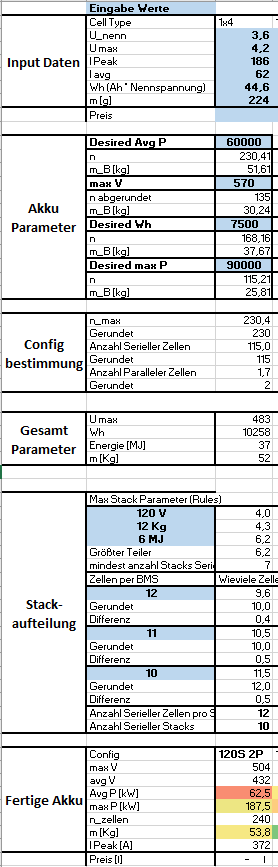
\includegraphics[width=0.2\linewidth]{bilder/Ausschnitt_zellvergleich}
	\caption{Ausschnitt aus der Zellauswahl Excel}
	\label{fig:Ausschnitt_zellvergleich}
\end{figure}

Unter dem Punkt Input Daten werden die Zellparameter aus dem Datenblatt der Zelle angegeben. Unter den Akkuparametern werden nun die Zielbedingungen bzw., Grenzwerte für den Akku bestimmt. Die min Avg. P. ist hierbei ein Parameter für die im Endurance angestrebte Leistung, die max.V ergibt sich aus der Spannungsfestigkeit des \ac{TS}, besonders relevant sind hierbei die Elektromotoren. Die min. Wh geben die mindestens vorgesehene Akkukapazität vor und die min. max. P. die angestrebte maximale Leistung die der Akku leisten muss. Aus diesen Parametern wird folgend eine minimal benötigte Zellanzahl bestimmt. Unter dem Punkt Akkuconfig wird nun die vorherig höchste bestimmte Zellanzahl ermittelt und gerundet. Hieraus bestimmen wir nun die Anzahl der parallel und seriell verschalteten Zellen und runden auf ganze Zellen.\\
Dies ergibt dann einige Gesamtparameter für den akku.\\
Unter dem Abschnitt Stackaufteilung werden die Zellen jetzt nach den Parametern des Regelwerkes möglichst optimal in Stacks aufgeteilt. Der Zielwert hierbei ist es, dass die tatsächliche Anzahl an Akkuzellen größer ist als die vorher errechnete benötigte Anzahl, es wird also aufgerundet. Weiter soll möglichst eine gerade Anzahl an Stacks herauskommen so das sich die Stacks im Akku möglichst leicht verteilen lassen. Hierbei können wir drei verschiedene Anzahlen von Zellen pro \ac{AMS} vorgeben die analysiert werden sollen.\\
Schlussendlich ist das Ergebnis ein fertig konfigurierter Akku. Diese Konfigurationen können nun gegenübergestellt und die Anzahl der weiter zu analysierenden Zellen eingegrenzt werden.\\
\\
Zur weiteren Analyse wurde auf Messdaten zurückgegriffen welche auf den Internetseiten dampfakkus.de und lygte-info.dk bereitgestellt wird. Aus diesen Daten ergeben sich folgende 2 Diagramme.

\begin{figure}[h]
	\centering
	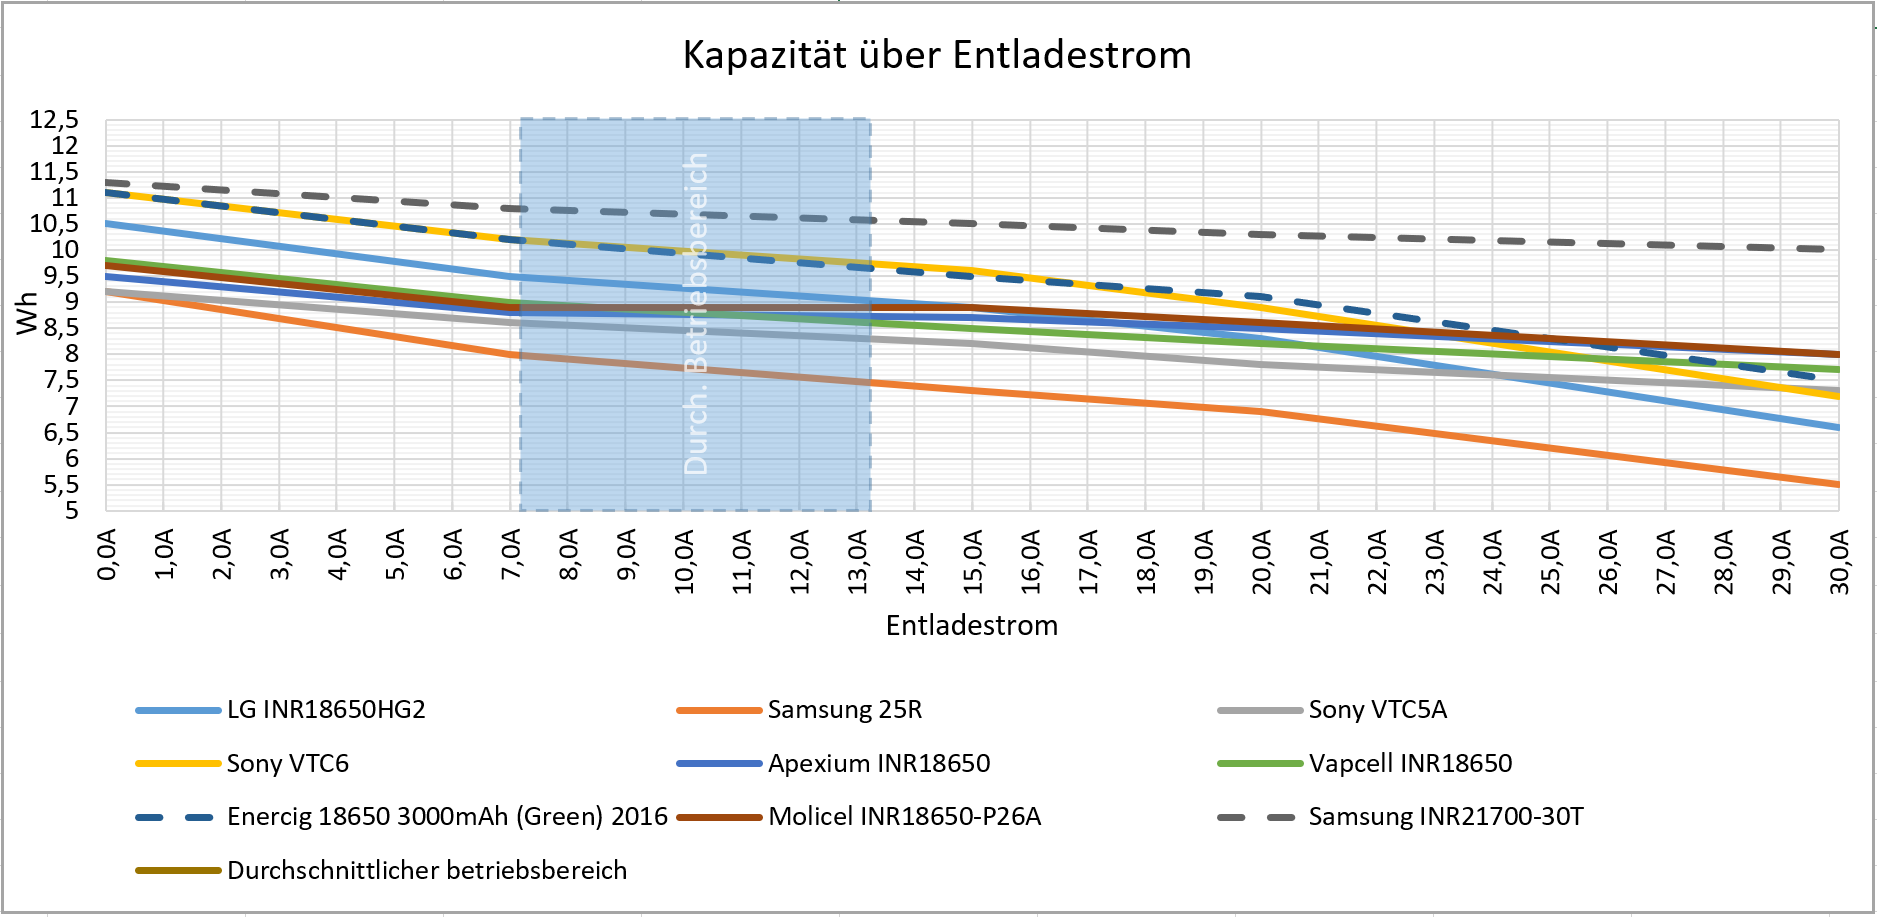
\includegraphics[width=0.6\linewidth]{bilder/Kapazitaet_ueber_Entladestrom}
	\caption{Kapazität über Entladestrom}
	\label{fig:Kapazitaet_ueber_Entladestrom}
\end{figure}

\begin{figure}[h]
	\centering
	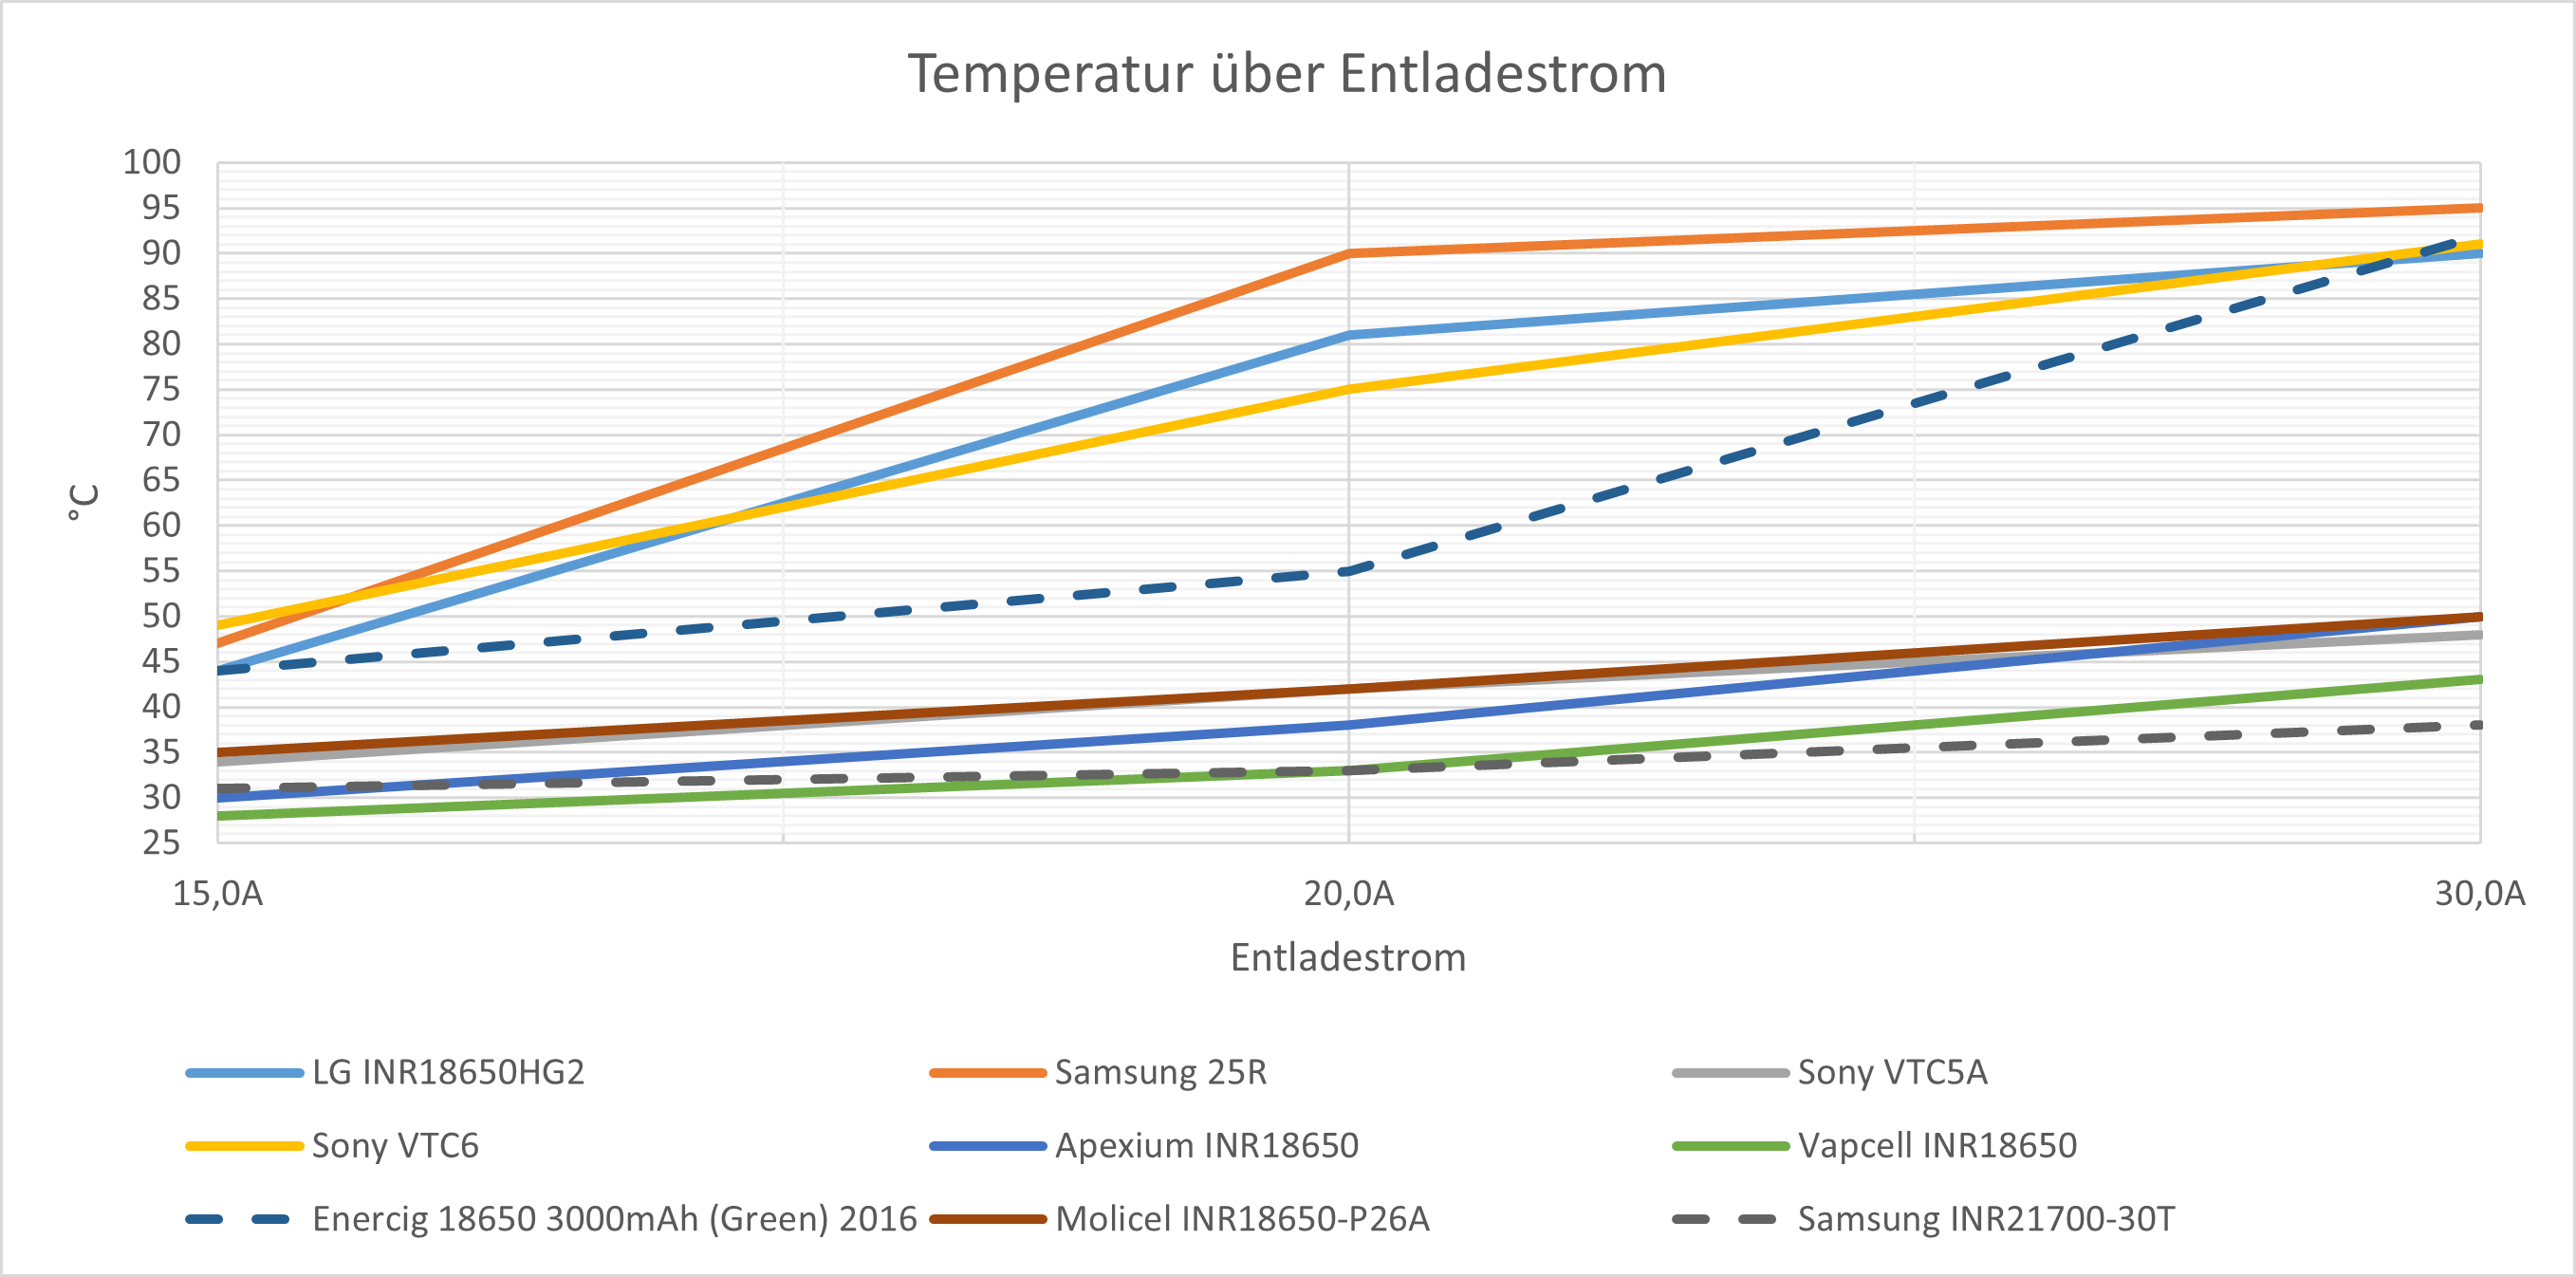
\includegraphics[width=0.6\linewidth]{bilder/Temperatur_ueber_Entladestrom}
	\caption{Temperatur über Entladestrom}
	\label{fig:Temperatur_ueber_Entladestrom}
\end{figure}

Das erste Diagramm ermöglicht es einen Eindruck von der Entladeeffizienz des Akkus, besonders bei hohen Strömen zu bekommen. Das Optimum wäre hier eine Horizontale Linie am oberen Rand des Diagramms. Hierbei sticht die Samsung INR21700-30T besonders hervor.\\
Das zweite Diagramm ermöglicht uns einen Eindruck von der thermischen Performance zu erlangen. Laut Regelwerk der Formula Student darf keine Akkuzelle zu einem Zeitpunkt die 60°C Marke überschreiten. Nichtbeachten führt zur Disqualifikation. hierbei sticht auch die vorher genannte Samsung Zelle hervor als auch die Vapcell INR18650\\
Hierbei vergleichen wir Rundzellen von verschiedenen Baumaßen, ein Vollständiger Akku mit den Samsung INR21700-30T wäre 7Kg schwerer als einer mit der Sony VTC6. Daher müssen am Ende alle erlangenden Erkenntnisse Berücksichtigt werden.

%evtl. netzgrafik von den top 2 oder 3 zellen machen. als finale gegenüberstellung 
\FloatBarrier
\subsubsection{Elektrisches Modell der Zelle}
Das Elektrische Modell ist für die Modellierung in der \ac{LTS} relevant. Hierbei werden die Limitierungen die sich aus dem Akku und dem restlichen Antriebsstrang ergeben simuliert. Ein Beispiel ist die sinkende Antriebsleistung bei abfallen der Spannung durch sinkenden \acfirst{SOC}. Das aktuelle Modell greift dabei auf zwei Datensätze zu um das verhalten zu modellieren. Einmal die Entladeeffizienz bzw. einen korrigierten Entladestrom, als auch auf ein Spannungskennfeld über den Entladestrom und \ac{SOC}. Die folgenden Abbildungen \ref{fig:Entladeeffizienz_VTC6} und \ref{fig:Spannung_ueber_SOC_Strom} gelten für die Sony VTC6. Die Daten entstammen wieder der Webseiten dampfakkus.de und lygte-info.dk.
\begin{figure}[h]
	\centering
	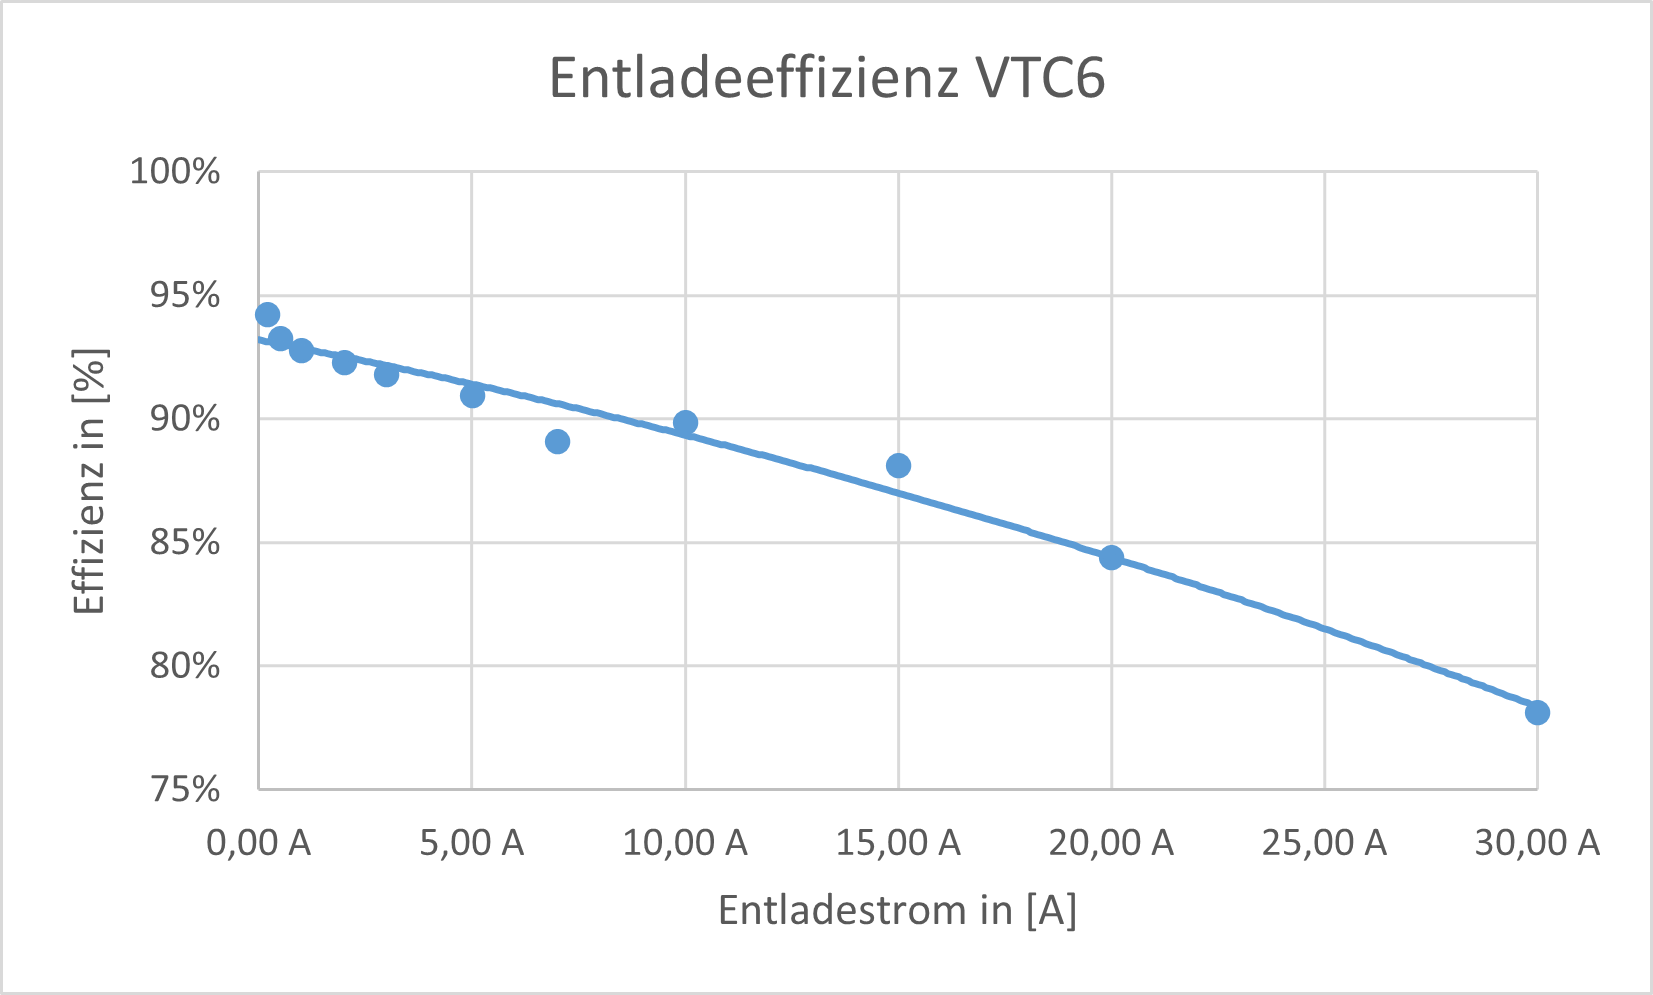
\includegraphics[width=0.7\linewidth]{bilder/Entladeeffizienz_VTC6}
	\caption{Entladeeffizienz VTC6}
	\label{fig:Entladeeffizienz_VTC6}
\end{figure}
\begin{figure}[h]
	\centering
	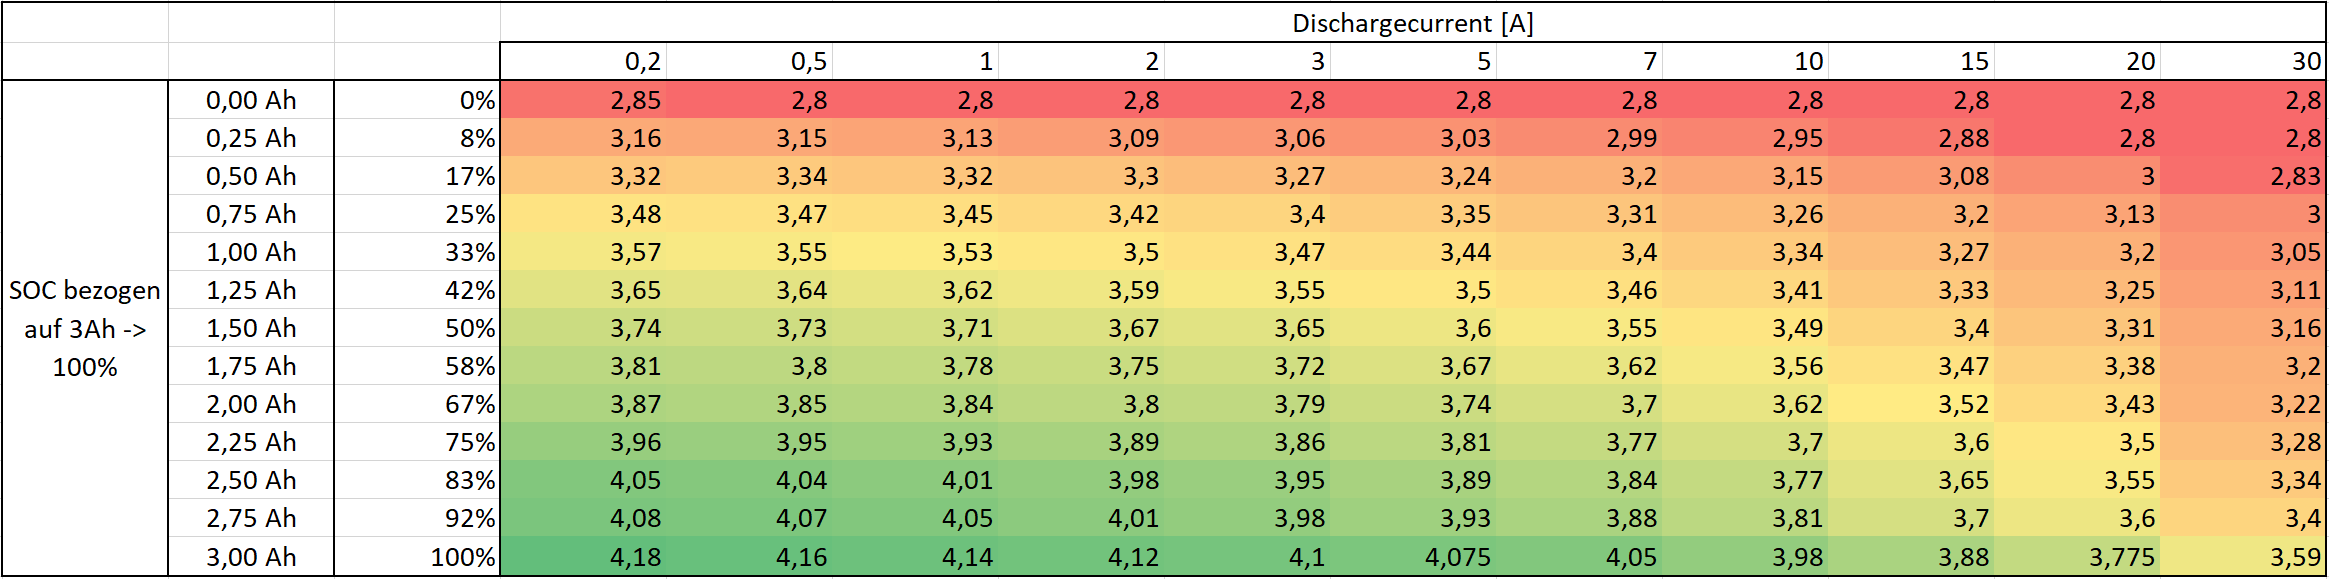
\includegraphics[width=0.7\linewidth]{bilder/Spannung_ueber_SOC_Strom}
	\caption{Spannungskennfeld VTC6}
	\label{fig:Spannung_ueber_SOC_Strom}
\end{figure}
\FloatBarrier
\subsubsection{Temperaturmodell der Zelle}
%Quelle!!!
Auf Basis der Masterarbeit Experimentelle Untersuchung von Batteriesystemen im simulierten niedrigen Erdorbit von Agnes Klein an der Universität Stuttgart konnte ich ein simples thermisches Modell der Akkuzelle erstellen. Bei dieser Arbeit wurde unter anderem die Akkuzellen des Types VTC6 innerhalb einer Thermal Vakuum Kammer betrieben und die thermischen Paramter der Zelle ermittelt. In folgender Grafik \ref{fig:parameterthermischesmodellvtc6} finden sie die dabei ermittelten Parameter.

\begin{figure}[h]
	\centering
	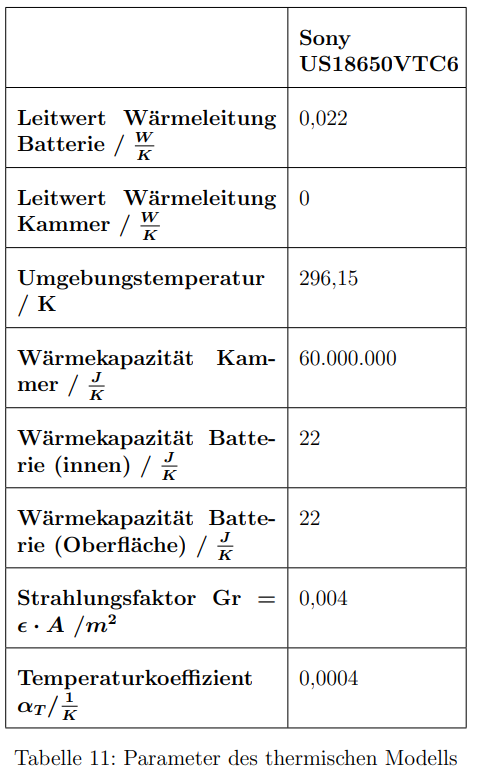
\includegraphics[width=0.4\linewidth]{bilder/Parameter_thermisches_modell_VTC6}
	\caption{Parameter des thermischen Modells der VTC6}
	\label{fig:parameterthermischesmodellvtc6}
\end{figure}

Damit ergibt sich folgende Gleichung.

\begin{equation}
	\glsc{symb:T_celli+1} = (\glsc{symb:I_cell}^2 * \glsc{symb:R_cell} - \glsc{symb:G_th} * (\glsc{symb:T_celli} - \glsc{symb:T_u}) - \glsc{symb:G_r} * \glsc{symb:SBoltz} * (\glsc{symb:T_celli} - \glsc{symb:T_u})^4) * \dfrac{1}{\glsc{symb:C_B} * \glsc{symb:m_Cell}} + \glsc{symb:T_celli}
\end{equation}

Mit dieser Gleichung ergeben sich folgende Kurvenverläufe für eine Auswahl von Entladeströmen.

\begin{figure}[h]
	\centering
	\includegraphics[width=0.7\linewidth]{bilder/temperatur_über_energie_vtc6_thermo_modell}
	\caption{Temperatur über Energieverbrauch VTC6}
	\label{fig:temperaturuberenergievtc6thermomodell}
\end{figure}
%Quelle
Mithilfe der Grafik \ref{fig:messdatenvtc6-temperatur-kapazitat-spannung} von der Universität BRNO (MATEC Web of Conferences 313, 00045 (2020)) können wir einen Plausibilitätscheck durchführen. Wir haben hier Messdaten von der Sony VTC6. Hierbei sind jedoch die Testbedingungen unbekannt.

\begin{figure}[h]
	\centering
	\includegraphics[width=0.7\linewidth]{"bilder/Messdaten_VTC6_ temperatur kapazität spannung"}
	\caption{Messdaten BRNO Temperatur über Energieverbrauch}
	\label{fig:messdatenvtc6-temperatur-kapazitat-spannung}
\end{figure}

Wir sehen, dass das erstellte Modell für den 10 A Graphen um ca. 3°C abweicht. Weiterhin sehen wir das bei der 20 A Linie die 90°C ca. 0,5 Ah früher erreichen. Diese Abweichungen sind nicht insignifikant, zeigen jedoch das unser Modell eher zu hohe als zu niedrige Temperaturen ausgibt was für die Zuverlässigkeit des Fahrzeuges positiv ist, da eine Auslegung der Kühlung mit diesem Modell wahrscheinlich zu einer Überkühlung und damit zu einem zu hohen Gewicht des Kühlsystems führt was für das erste Fahrzeug kein sonderlich großes Problem darstellt. Die Abweichung dürfte darauf zurückzuführen sein das die Modellparameter im Vakuum ermittelt wurden und insofern Wärmeübertragung durch Konvektion etc. nicht berücksichtigt werden konnte. Um diesem Sachverhalt weiter auf den Grund zu gehen wurde im Anschluss eine Simulation mit Ansys Fluent durchgeführt.

\begin{figure}[h]
	\centering
	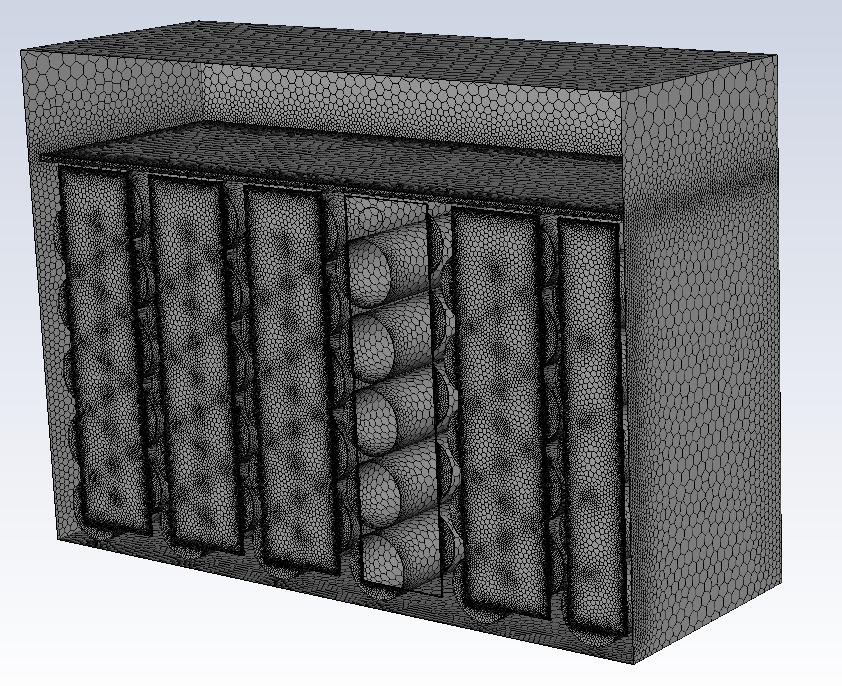
\includegraphics[width=0.7\linewidth]{bilder/Accu_Sim_therm_7_2A_45min_simple_mesh}
	\caption{Mesh der Multiphysik Fluent Simulation des Akkustacks}
	\label{fig:accusimtherm72a45minsimplemesh}
\end{figure}

\begin{figure}[h]
	\centering
	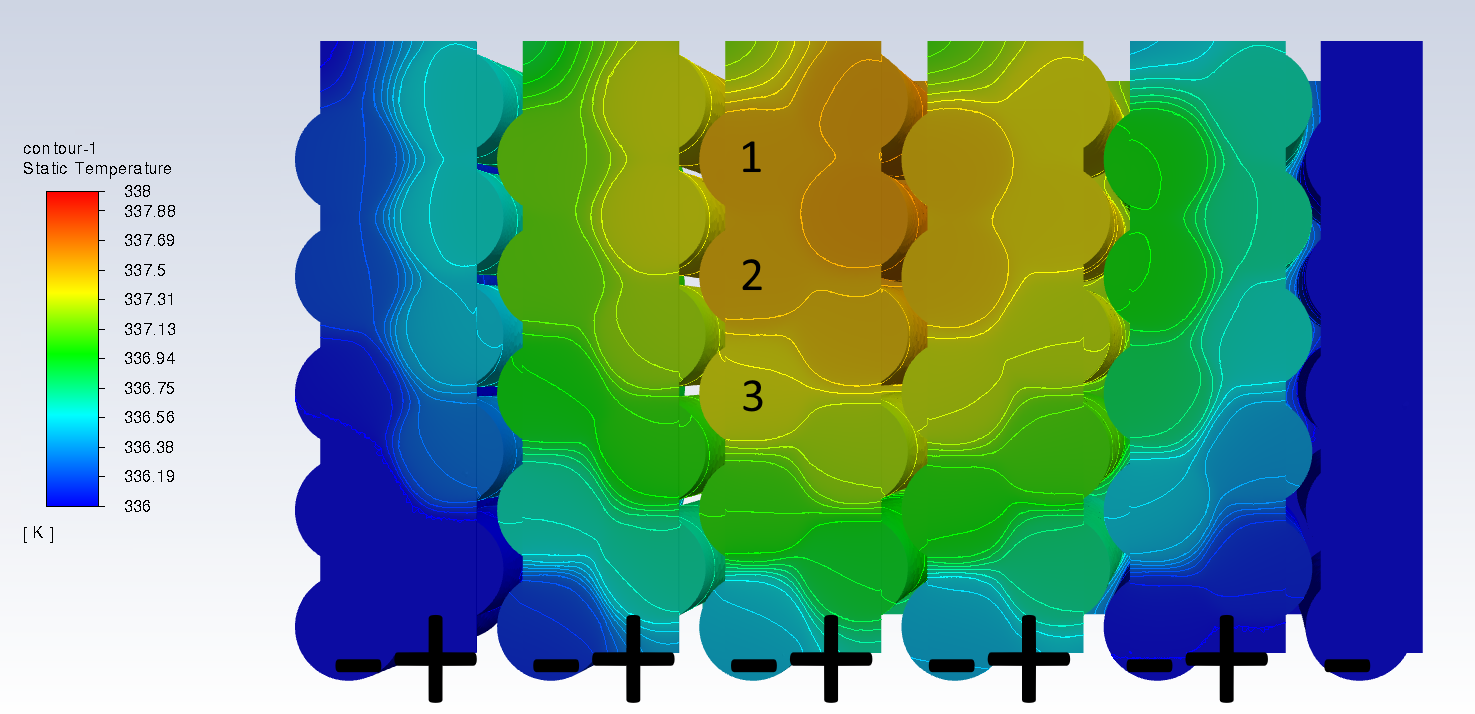
\includegraphics[width=0.7\linewidth]{bilder/Accu_Sim_therm_7_2A_45min_simple}
	\caption{Multiphysik Simulationsergebnis Akkustack}
	\label{fig:accusimtherm72a45minsimple}
\end{figure}

In dieser Simulation wurde ein gesamter Akkustack in seinem Gehäuse simuliert. Dabei wurde mit einem konstanten Strom von 7,2 A simuliert. Dieser Strom ergibt sich aus der r\ac{LTS} siehe sectrion?????. Die Simulation wurde für 32 min laufen gelassen um ein gesamtes Endurance darzustellen. Ziel der Simulation ist es die Effekte der Konvektion zu berücksichtigen, aber auch zu sehen inwiefern sich die Zellen gegenseitig beeinflussen. Allerdings wurden auch diverse Vereinfachungen getroffen insofern das die Akkuzellen sich uniform aufwärmen. In der Realität dürfte man am negativen Pol der Akkuzelle eine deutlich höhere Temperatur feststellen können als auf der positiven Seite. Weiterhin wurden diverse Teile wie die elektrische Isolierung etc. weggelassen da dies den Simulationsaufwand sonst erheblich vergrößert hätte. Mit den vorliegenden Vereinfachungen lief die Simulation für 46 Stunden.\\
Zur Analyse, wir sehen nach der Simulationszeit eine Höchsttemperatur von 64,85°C und eine Tiefsttemperatur von 62,85°C. In dieser Hinsicht stimmt die Ansys Simulation eher mit der 10 A kurve aus unserem Modell zusammen als mit den Messdaten. Zusammengefasst stellt man fest das definitiv weitere Arbeit in diesem Themenbereich von Nöten wäre, um zu einer optimalen Lösung zu kommen, dies jedoch aufgrund des engen Zeitplanes und des enormen anderweitigen Aufwandes nicht möglich ist.

\FloatBarrier
\subsubsection{Der Stack Aufbau} %(mit Tim)%

Für die Konstruktion des Akkustacks gab es im Laufe der Saison viele Iterationen. Die folgend erläuterte ist eine Optimierte Version derer die für den TY22 gebaut wurde.

\begin{figure}
	\centering
	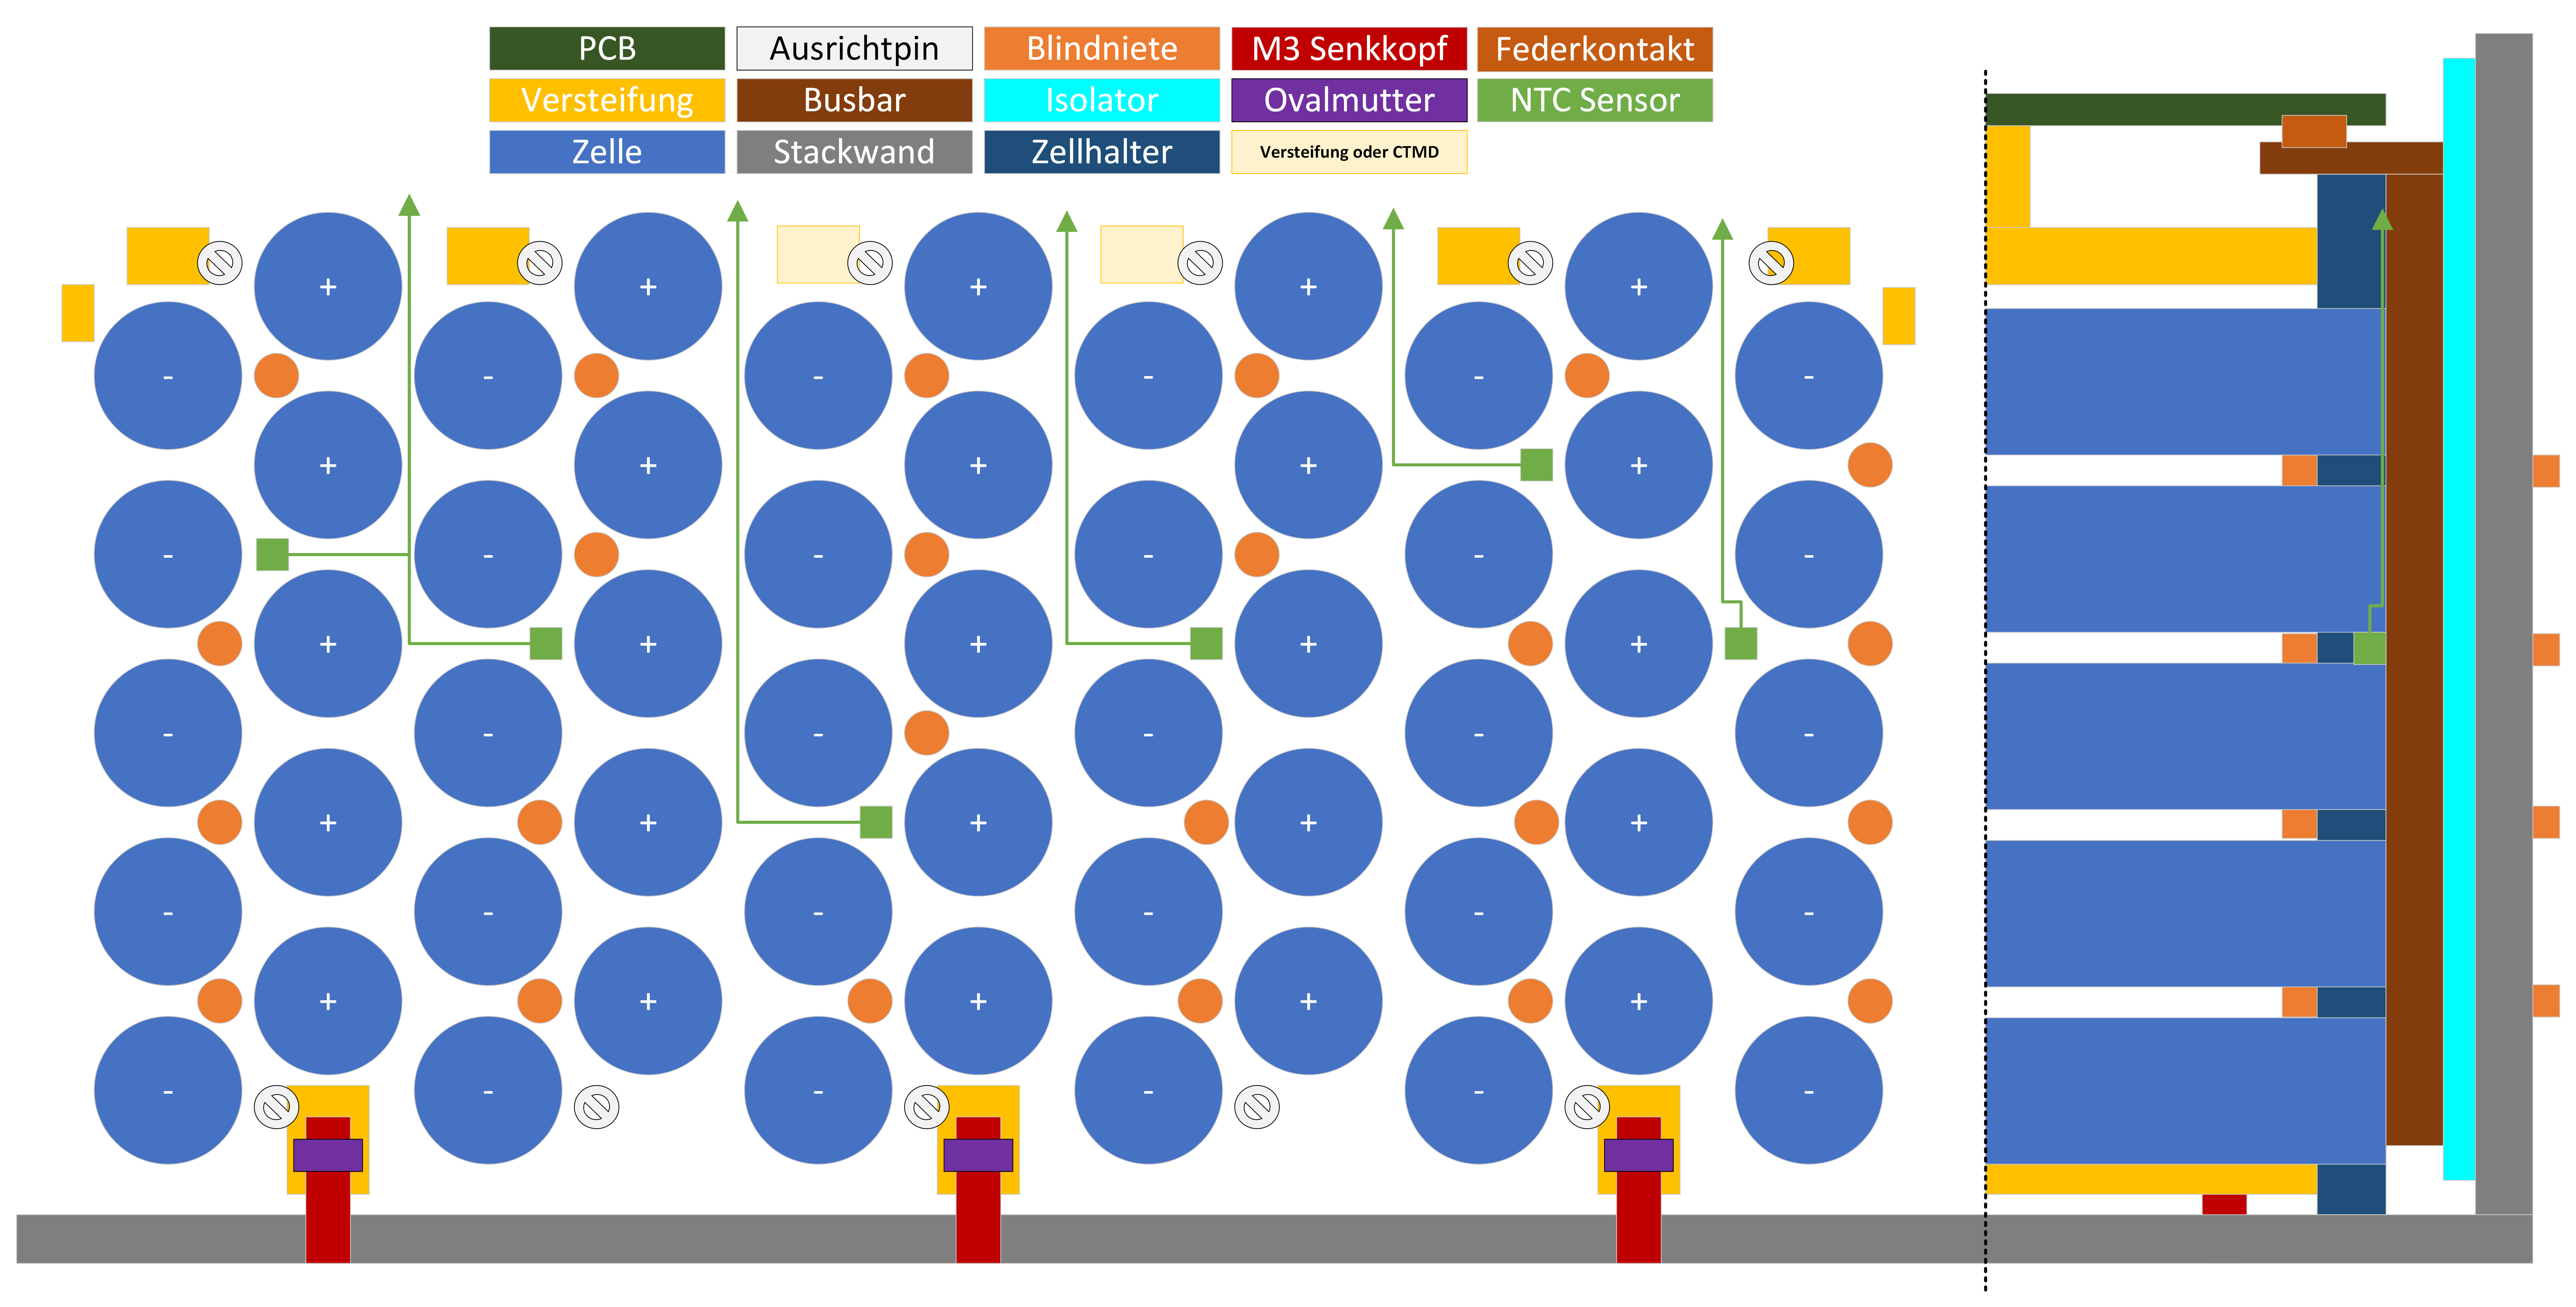
\includegraphics[width=0.7\linewidth]{bilder/Stackaufbau_Prinzipskizze}
	\caption{Prinzipskizze Stackaufbau}
	\label{fig:stackaufbauprinzipskizze}
\end{figure}

\begin{figure}
	\centering
	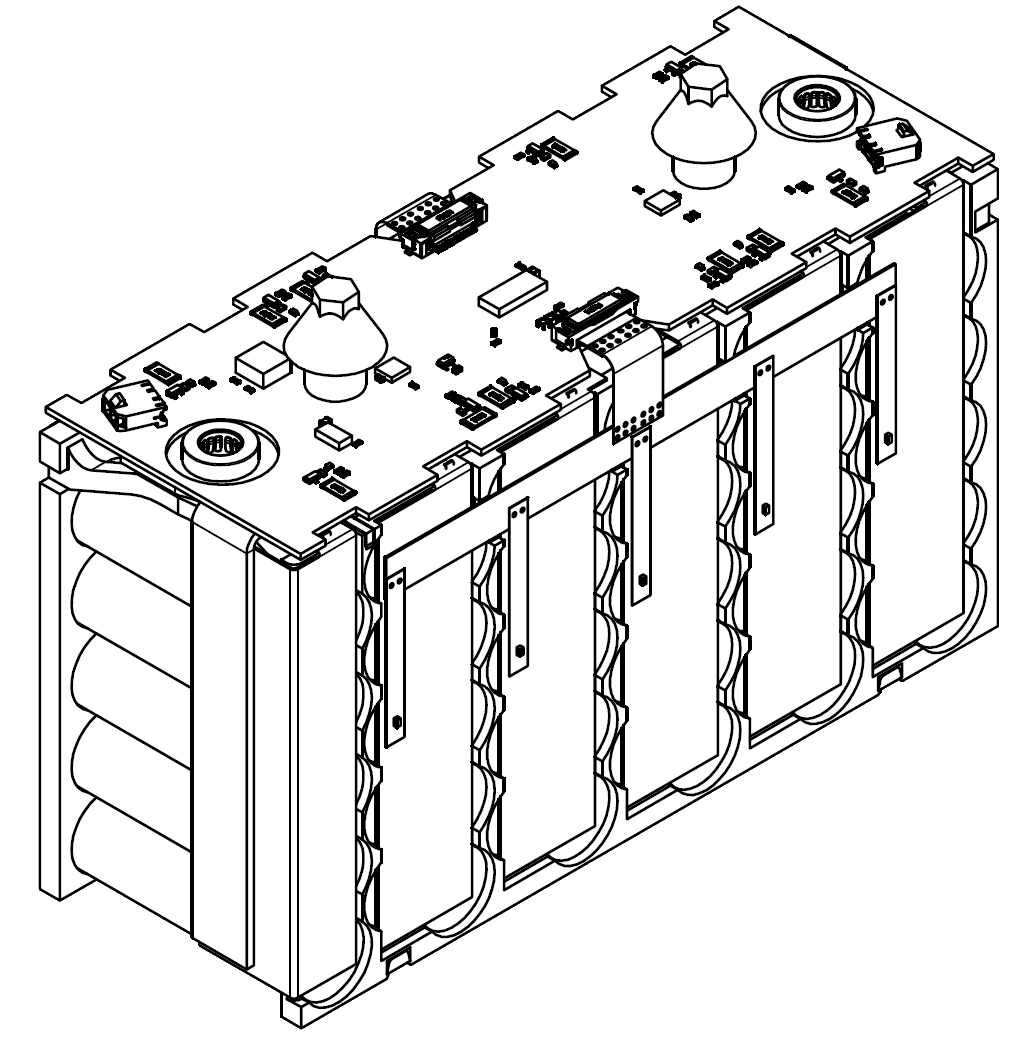
\includegraphics[width=0.7\linewidth]{bilder/Stach_for_EDR}
	\caption{Iso Ansicht Stack Baugruppe}
	\label{fig:stachforedr}
\end{figure}



Die Zellen sind liegend in Fünferpaketen gestapelt und mit einem Versatz aneinander gereiht um den Leerraum zwischen den Zellen möglichst klein zu halten. Die Busbars verbinden immer ein 5er Negativpole mit einem 5er positiv Pole. Zusätzlich befinden sich in der nähe der Zellen 2 Ausrichtpins um die Busbar auf dem Stack bei der Montage positionieren zu können. Der Aufbau auf den Polen besteht aus einer angeschweißten Busbar, darauf folgt ein abriebfester Isolator, und dann die Trennwand des Akkus. nach Innen haben wir noch einen 3D gedruckten Halter in dem die Akkuzellen ausgerichtet werden. Dieses ganze Paket wird mit Blindnieten vernietet. Ziel hierbei ist es einen möglichst guten thermischen Kontakt von den Polen der Zelle zum Akkugehäuse herzustellen. Selbiges ist aus Aluminium und Flächig mit dem Monocoque verschraubt welches auch aus Aluminium gefertigt ist. dies ergibt eine riesige thermische Masse und stellt so eine Kühlung für den Akku bereit. Die Stack-Seitenwand liegt als L-Profil vor, und wird anschließend mit dem Akkuboden mit Hilfe von M3 Senkkopfschrauben und Ovalmuttern verschraubt. In diesem Zuge sind in die 3D gedruckten Querversteifungen im Stack Ovalmuttern eingeklebt. Diese Querversteifung sorgen einerseits für mechanische Stabilität, stellen aber auch Anbindungspunkte für den \ac{AMS}-Slave als auch für die Maintenance Plug Steckverbinder bereit. Die Busbar ist auch als L-Profil ausgeführt und lappt oben über den Stack über, diese Finnen werden seitens des \ac{AMS}-Slaves mit Hilfe von Federkontakten kontaktiert um eine Verbindung für die Spannungsmessung als auch das Balancing herzustellen. Die \acfirst{NTC}-Sensoren befinden sich in den Leerstellen wo keine Nieten benötigt werden, immer eine Niete mittig in drei Zellen. Die \ac{NTC}`s sind rückseitig auf die Busbar geklebt. Um das Design günstig zu halten kann die Verbindung über 0,25 mm\^2 Kabel erfolgen, welche Sensorseitig auf Lötpads und \ac{AMS}-seitig in einen Stecker gebracht werden. Bei der Steckverbinderauswahl ist zu beachten das er über einen Verriegelungsmechanismus verfügt, und nicht zu klein ist. Besonders kleine Steckverbinder machen an der stelle die Verarbeitung schwer oder praktisch unmöglich. Präferiert wäre hier ein Flex-\acfirst{PCB}, dies ist jedoch \ac{idR} recht teuer. In dem Stackhalter müssen entsprechende Einkerbungen vorgehalten werden durch die die Kabel zu führen sind. In die Anbindung des \ac{AMS}-Slave ist ein Feature vorzusehen welches eine leichte Extraktion des Stacks aus dem Akku erlaubt, und bei der Konstruktion der Maintenance Plugs ist auf Ergonomie zu achten, so das ein Mensch mit einem \ac{HV}-Handschuh noch gefahrlos einen solchen ziehen kann. Weiter ist bei den Maintenance Plugs auf Verstecksicherheit zu achten. Ein letzter Punkt ist die Positionierung des \acfirst{CTMD}, also entweder des i-Button oder der kabelgebunden Sensoren mit Steuergerät, je nachdem was die \acfirst{FSG} verwenden möge. Hier ist besonders die Positionierung des \ac{CTMD} am Hotspot schwer nachzuweisen. Eine Simulation kann hier eine Richtung aufzeigen, stellt jedoch einen großen Zeitaufwand dar und ist im allgemeinen so ungenau (ohne signifikanten Zeitaufwand), dass sich nur sehr begrenzt belastbare Aussagen hiermit treffen lassen.

\FloatBarrier
\subsubsection{Die Busbar}
 Bei der Auswahl der Materialien für die Busbar sind die Masse als auch die elektrische, respektive die thermische Performance ausschlaggebend. Ein weiterer Maßgebender Faktor sind die möglichen Fertigungsverfahren um den Kontakt zwischen Zelle und Busbar herzustellen. Folgende Grafiken ergeben sich aus den Materialkonstanten und der Erwärmung über den Widerstand der Busbar bei dem entsprechenden Strom und über die Wärmekapazität und die Betriebszeit.
 
 \begin{figure}[]
 	\centering
 	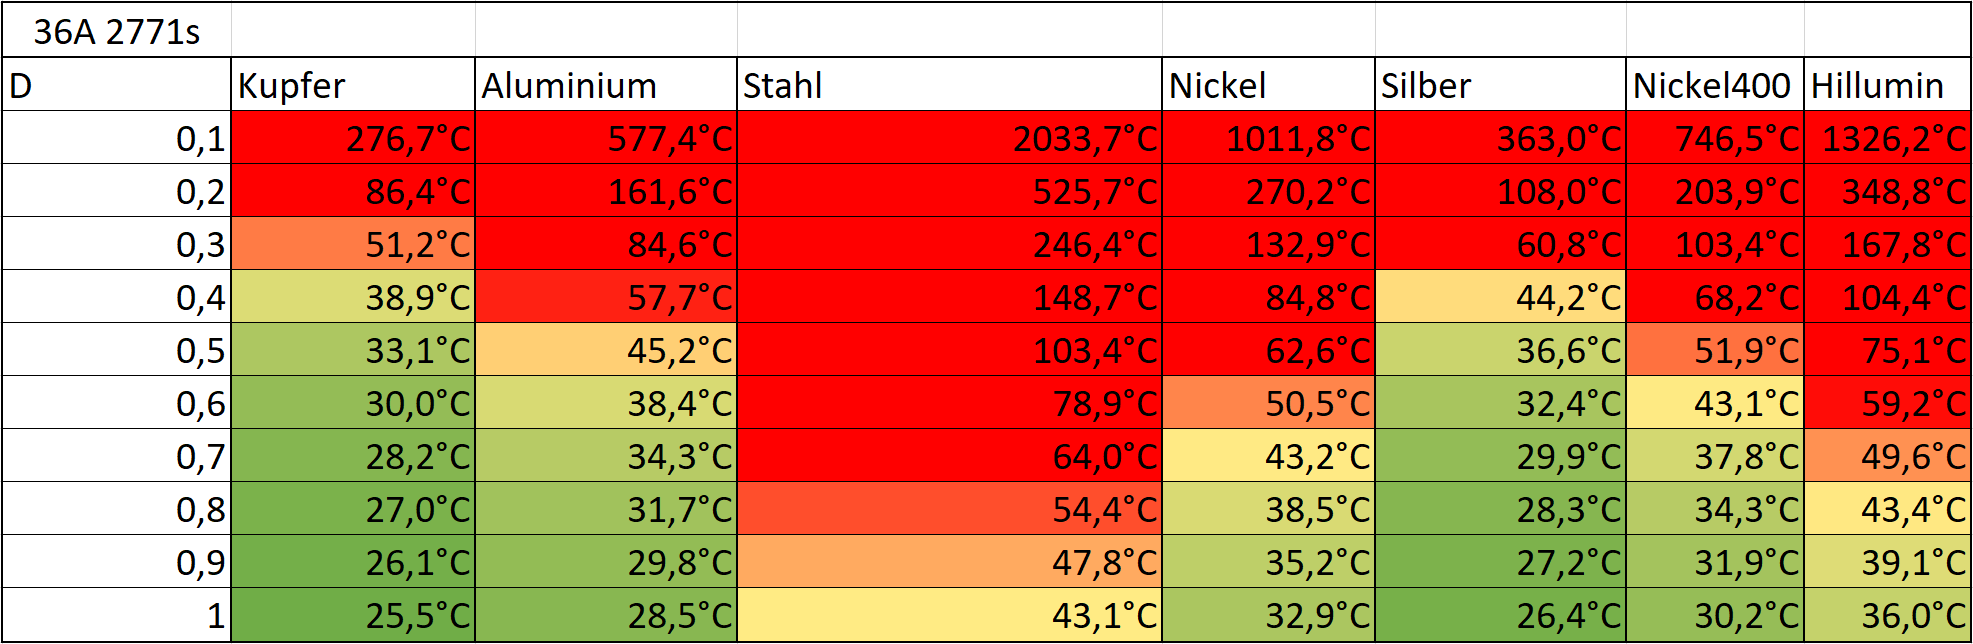
\includegraphics[width=0.7\linewidth]{bilder/Busbar_temp_36A_2771s}
 	\caption{Busbartemperatur bei 36 A und 2771 s}
 	\label{fig:Busbar_temp_36A_2771s}
 \end{figure}
\begin{figure}[]
	\centering
	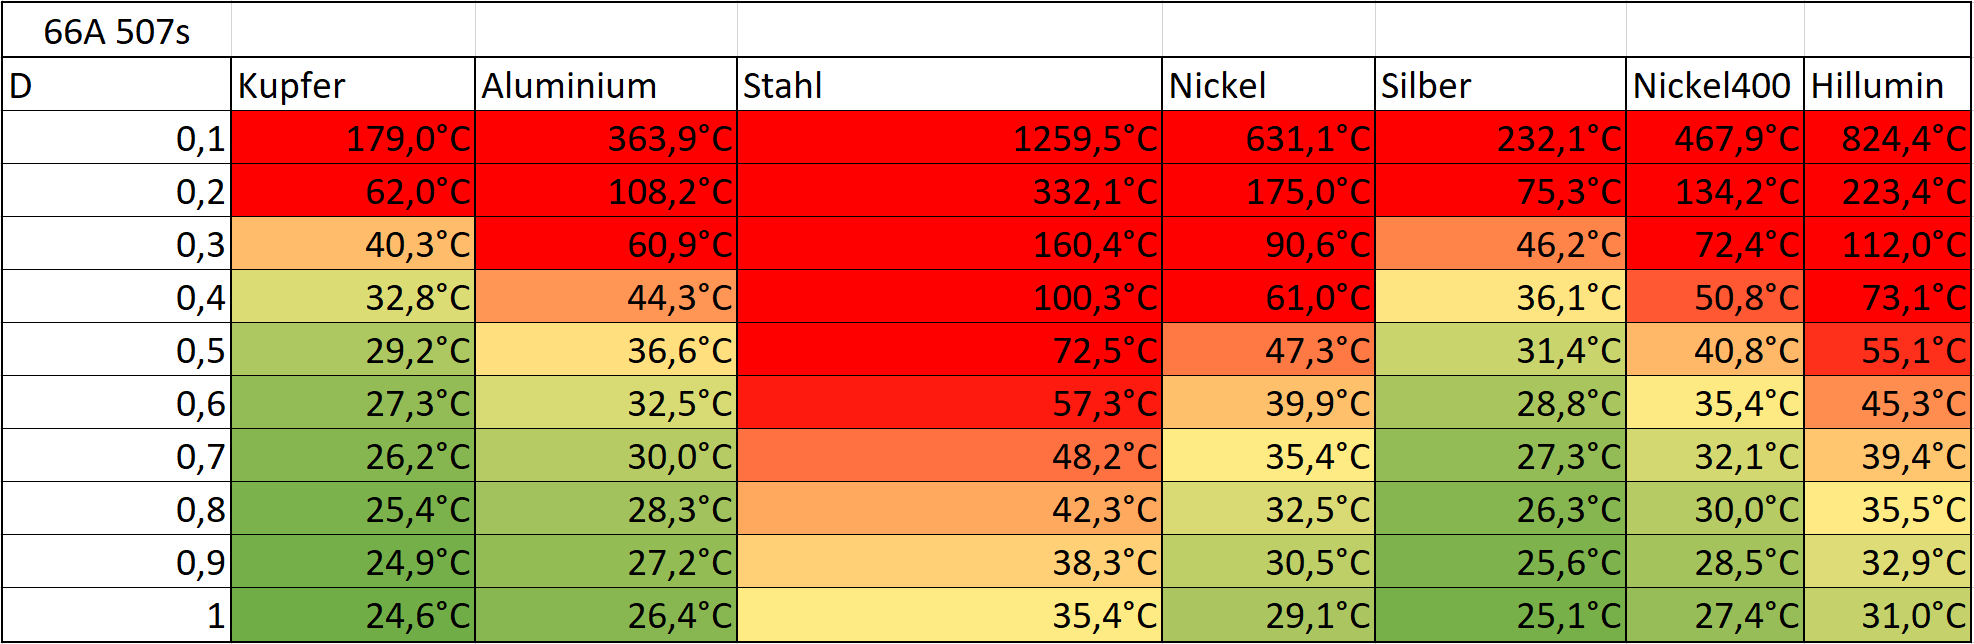
\includegraphics[width=0.7\linewidth]{bilder/Busbar_temp_66A_507s}
	\caption{Busbartemperatur bei 66 A und 507 s}
	\label{fig:Busbar_temp_66A_507s}
\end{figure}
\begin{figure}[]
	\centering
	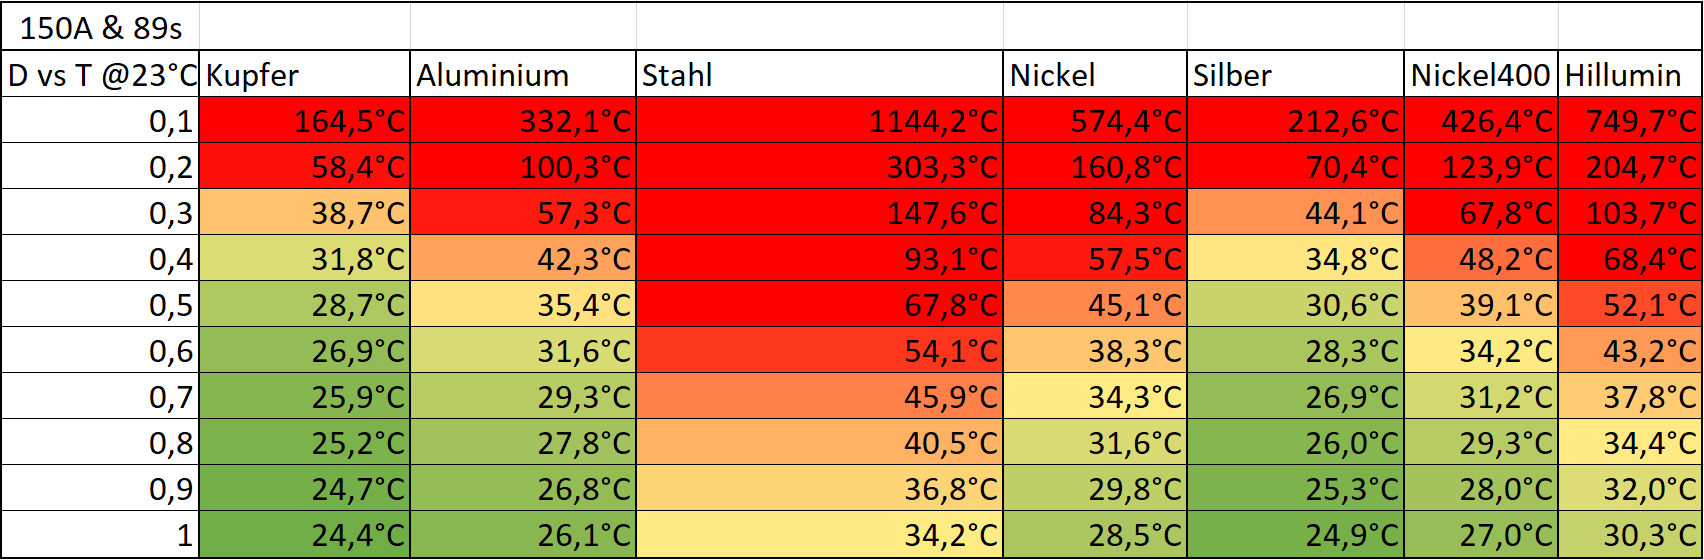
\includegraphics[width=0.7\linewidth]{bilder/Busbar_temp_150A_89s}
	\caption{Busbartemperatur bei 150 A und 89 s}
	\label{fig:Busbar_temp_150A_89s}
\end{figure}

Es ist ersichtlich das Kupfer die beste thermische Performance in Bezug auf die Materialmenge bringt, aufgrund der niedrigen dichte Aluminium allerdings gravimetrisch mit Abstand die beste Performance zeigt. Nickel, respektive Nickel400 liegen jedoch nicht weit zurück, lediglich stahl lässt sich aufgrund der Ergebnisse direkt ausschließen.\\
\\
In Bezug auf die Fertigung ergeben sich bei Rundzellen zwei Wege, einmal das Schweißen aber auch die Federkontaktierung.\\
Die Kontaktierung über eine Feder an eine Rundzelle sollte dem Leser hinreichend aus anderen batteriebetriebenen Geräten bekannt sein. Hierbei ergeben sich schnell einige Fragestellungen. Einmal die Frage nach der Ermittlung des Übergangswiederstandes. Einflussfaktoren sind die Anpresskraft, die Oberflächenrauigkeit, die Kontaktfläche, als auch der Materialmix. Eine Berechnung ist jedoch praktisch aufgrund des enormen Aufwandes und großer Unsicherheiten kaum möglich. Weiter stellt sich da die Frage wie groß z.b die max. mögliche Anpresskraft auf die Akkuzelle sein kann oder welche Oberflächenrauhigkeit ein Pol einer Akkuzelle mit sich bringt. Weiter ist die Relaxation ein Problem. Hierbei würde die Anpresskraft im Verlauf der Zeit abnehmen und damit der Übergangswiederstand steigen. All diese Parameter müssten in Versuchsreihen ermittelt und untersucht werden um auf ein sicheres System zu kommen. Das Verschweißen von Akkuzellen wird dabei gerade im Hochstrombereich bereits industriell angewandt und ist damit hinreichend bekannt.\\
Bei den Schweißverfahren teilt sich nun der Weg in das Laser bzw. \acfirst{WIG}-Schweißen und in das Punkt oder Widerstandsschweißen auf. Ersteres Verfahren ermöglicht das Verschweißen unterschiedlicher Metalle wie z.b Stahl an Aluminium oder Kupfer. Zweiteres Verfahren eignet sich nur für Materialien mit einem verhältnismäßig hohen elektrischen Widerstand da der Schweißpunkt durch die Temperaturentwicklung gebildet wird die entsteht wenn ein hoher Strom durch einen verhältnismäßig hohen Übergangswiederstand geleitet wird. Daher eignet sich das Widerstandsschweißen nur für Nickel oder Stahl. Die anderen Materialien sind nicht inhärent nicht geeignet, stellen aber besondere Anforderungen an den Prozess so das die Standard Geräte hier \ac{idR} nicht ausreichen. Systemparameter sind beim Widerstandsschweißen die Schweißspannung als auch der Schweißstrom und die Pulsdauer. Ein großer Nachteil des Laser bzw. \ac{WIG}-Schweißens ist das dieses Verfahren bisher nur im industriellen Maßstab angewandt wird und es keinerlei Geräte für den Hobbybedarf gibt. Dies führt dazu das diese Geräte \ac{idR} enorm teuer und schwer zu bekommen sind. Hierbei wäre es sicherlich möglich ein typisches \ac{WIG}-Schweißgerät für diese Zwecke zu modifizieren dies bringt jedoch wieder die entsprechende Unsicherheit in den Prozess. Punktschweißgeräte sind in diversen Ausführungen und Preisklassen gut erhältlich, dies aber nur aus dem Asiatischen Markt, wo die Geräte allem Anschein nach mit größeren Qualitätsproblemen zu kämpfen haben.
	
\FloatBarrier
\subsubsection{Der Akkumulator Container}

Der Akku besteht aus 12 Einzelstacks. Hierbei befinden sich 6 nebeneinander und davon 2 Reihen hintereinander. In der vorderen Sektion die unter den Fahrersitz ragt befinden sich die \ac{AIR}`s als auch die übrige Akkumulator Elektronik wie das \ac{IMD} der \ac{AMS}-Mster und der \ac{HV}-DCDC.
\begin{figure}
	\centering
	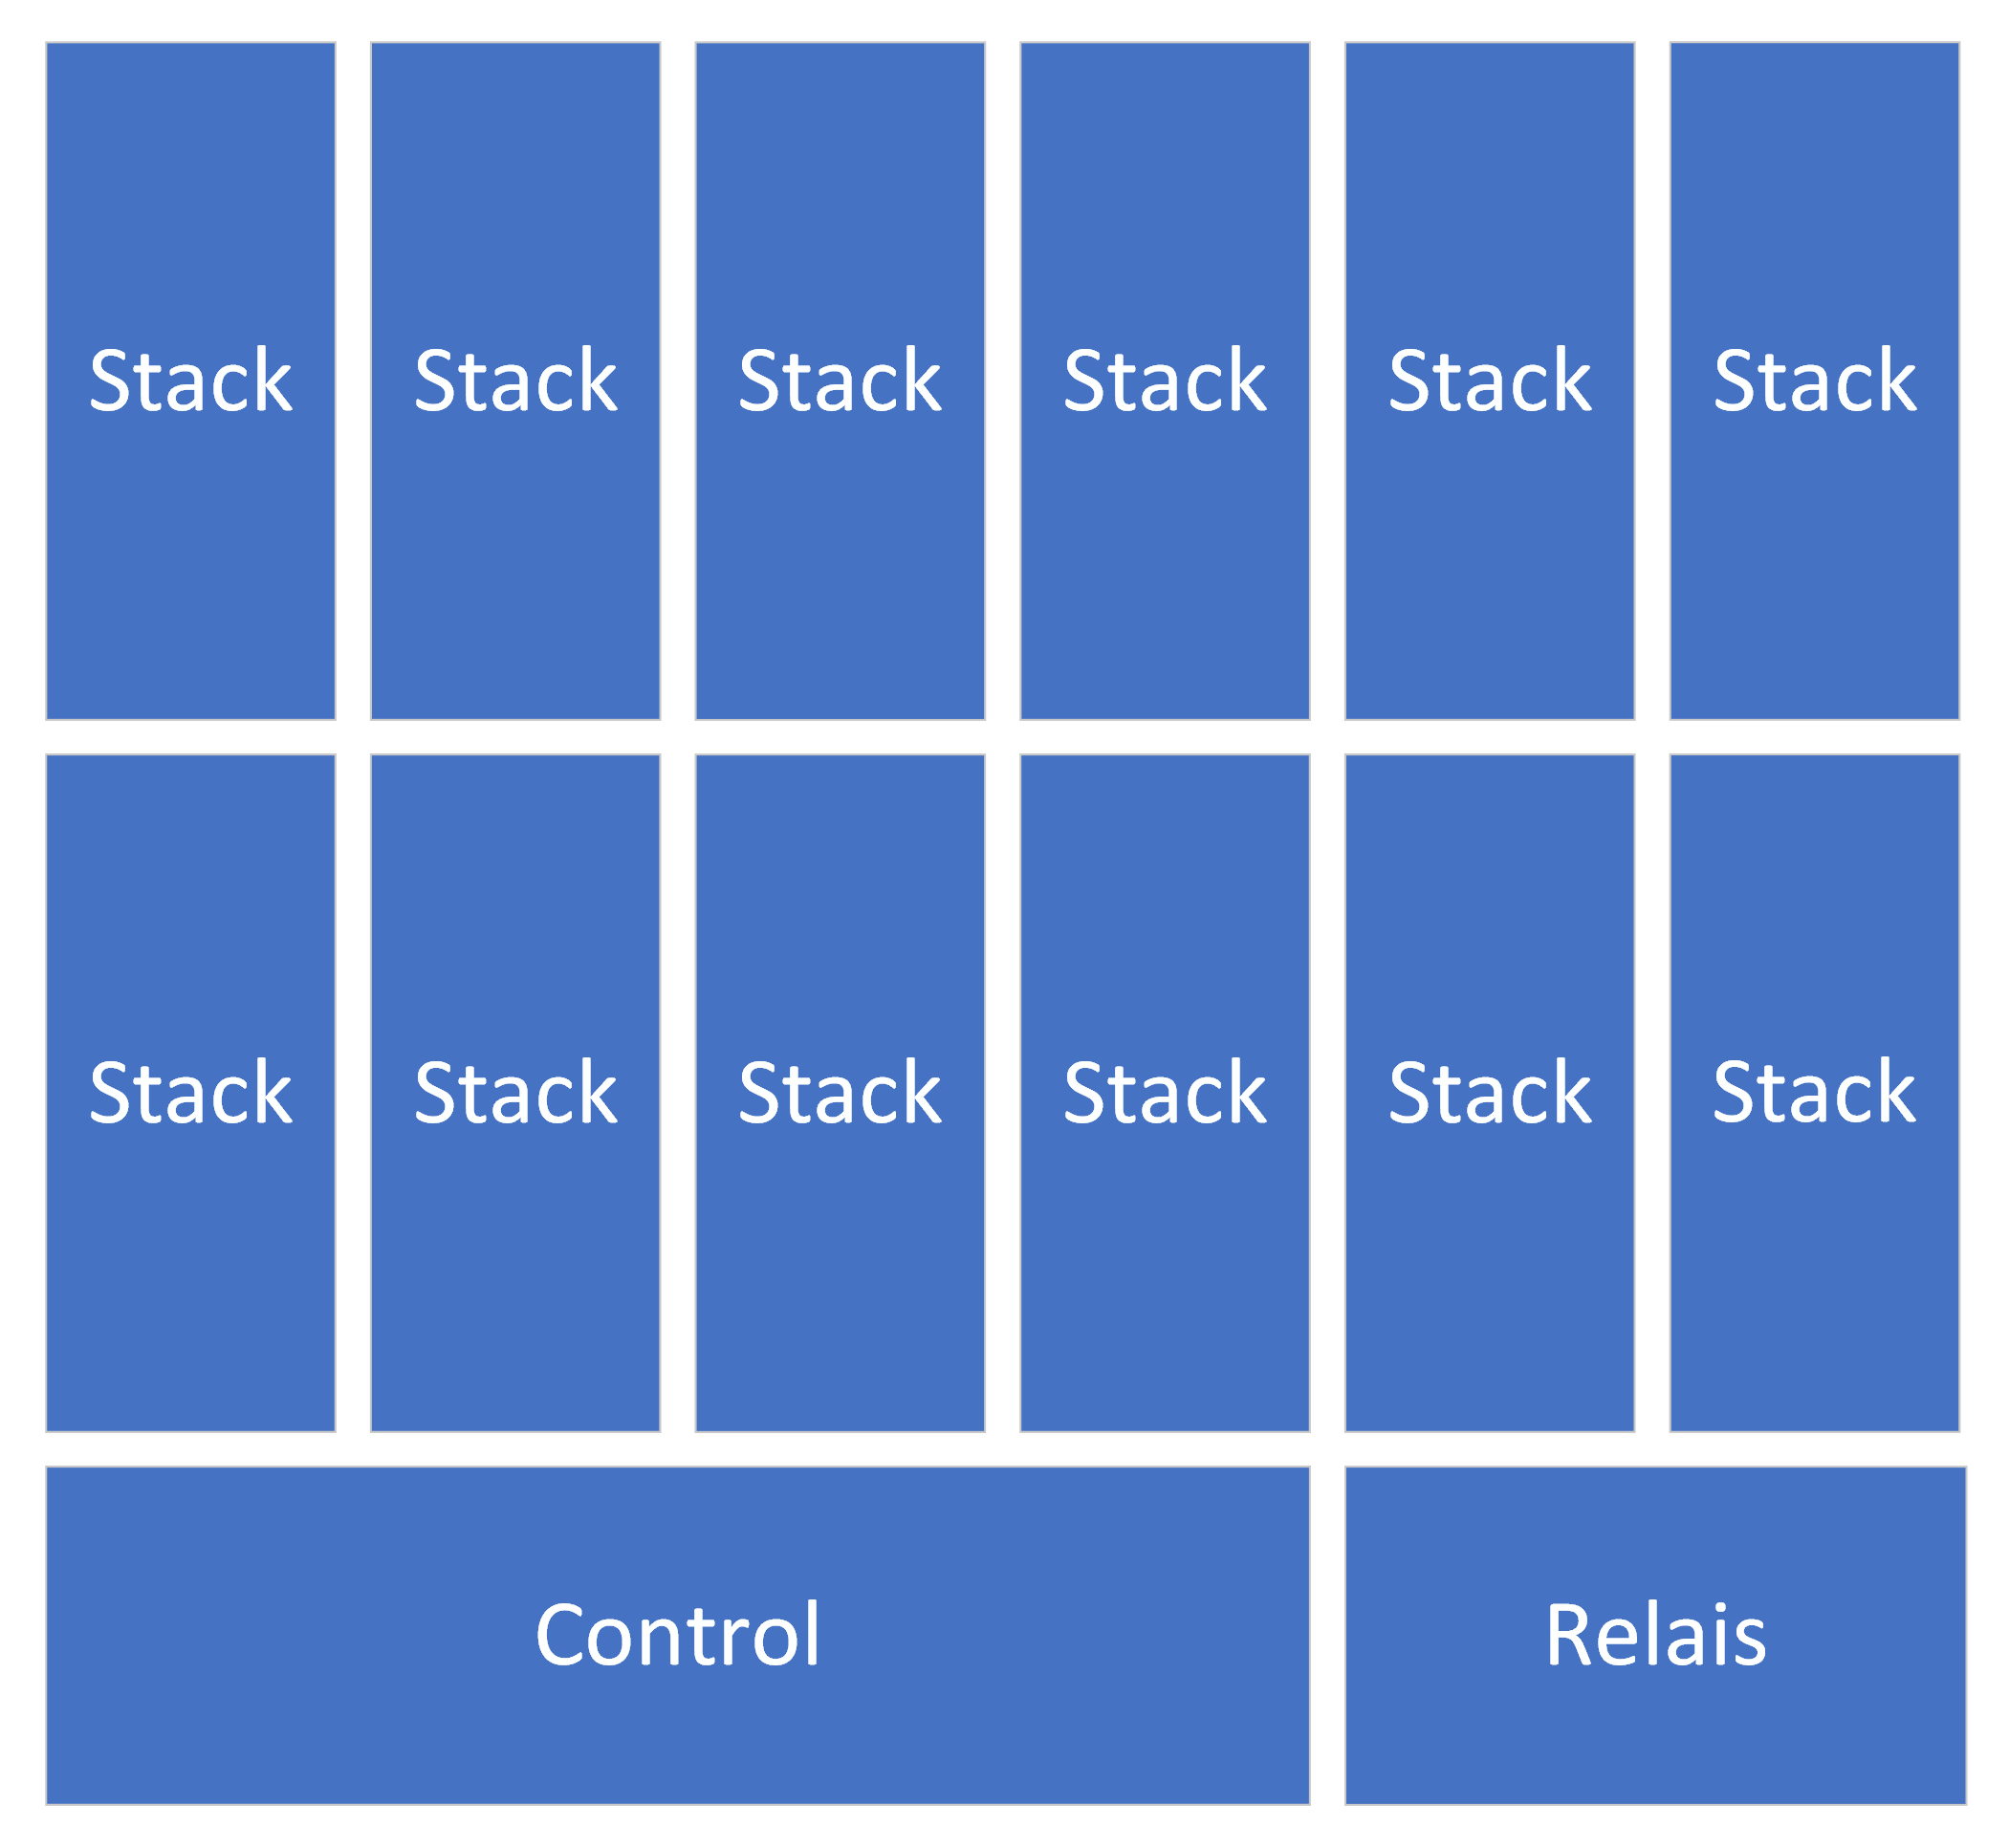
\includegraphics[width=0.7\linewidth]{bilder/Akku_Layout}
	\caption{Layout des Akkumulators}
	\label{fig:akkulayout}
\end{figure}
Der Akkumulatorcontainer besteht aus Aluminium. Dabei muss vom Regelwerk her der Boden mindestens 3,2 mm und die wände 2,3 mm Dick sein. Gewählt wurden respektive 4 mm und 2,5 mm. In der ersten Version handelt es sich bei dem Container um mehrere geschweißte Biegeteile. Solch ein Konstrukt zeichnet sich jedoch durch derart starken Schweißverzug aus das bei der Folgeversion eine Kombination aus Nieten kleben, schrauben und schweißen anzuraten ist. Gerade mit dem überarbeiten Stack Konzept lässt sich eine reine Schweißkonstruktion nicht mehr umsetzten. Hierbei währen die Stackwände vernietet und verschraubt, die Bodenwanne eine Biege-Schweißteil, der Deckel ein Biegeteil und etwaige interne Anbindung für z.b die \ac{HV}-Stecker sind geklebt.

!!Bild von aktueller CAD mit beschriftung!!

\section{Elektromotor}
Für die Auswahl des Elektromotors gibt es 5 verschiedene in der Formula Student allgemein anerkannte Lösungen. Diese werden nachfolgend erläutert.\\
\\
\textbf{Emrax}\\
Beim Emrax Motor handelt es sich um eine Axial Flux \acfirst{PMSM}. Zusammenfassend sind die Emrax Motoren sehr flach, haben aber einen großen Durchmesser. Sie zeichnen sich durch ein hohes Drehmoment und damit verhältnismäßig niedrige Drehzahlen aus, im Bereich von 7-8K \acfirst{RPM}. Sie sind nur in recht großen Formaten und damit großen Leistungen erhältlich so das ein 1 oder 2 Motoren Antriebskonzept realisierbar ist. Außerdem handelt es sich hierbei um eine reine Kauflösung. \\
\\
\textbf{AMK}\\
Die AMK Motoren sind Radial Flux \ac{PMSM}. Sie sind insofern eher lang und haben kleine Durchmesser. Die Bauform gleicht insofern eher dem klassischen Elektromotor. Sie zeichnen sich durch extrem hohe Drehzahlen aus, oberhalb der 20k und damit durch eine enorme Leistungsdichte. Sie sind in eher kleinen Leistungsbereichen zu bekommen so das beinahe nur ein Allradantrieb sinnvoll umsetzbar ist. Auch hierbei handelt es sich um eine reine Kauflösung. \\
\\
\textbf{Fischer}\\
Die Motoren von Fischer sind im großen und ganzen gleichzusetzen mit den AMK Motoren. Der große Unterschied ist das hier das Gehäuse selbst designt werden muss und alle Teile selber gefertigt werden müssen. Dies stellt große Herausforderungen die Fertigungstechnik da es sich dabei auch um 5-Achs gefräste Titanteile handelt.\\
\\
\textbf{Asia \& Co}\\
Eine weitere Optionen wäre es günstige Motoren eines Asiatischen Hersteller zu beschaffen, als Beispiel wäre hier die Firma Freerchhobby zu nennen, es gibt aber viele mehr. Diese Motoren zeichnen sich durch ein herausragend niedrigen Preis aus sowohl für den Motor als auch den zugehörigen Motorcontroller. Problematisch hierbei ist, das diese Motoren in der Regel nur bis Spannungsbereiche von 120 V verfügbar sind. Der dabei bei 80 kW resultierende Strom ist enorm. Heißt das entweder die Leistung zu reduzieren wäre oder die elektrische des Auslegung des \ac{TS} besondere Ansprüche gestellt hätte. Weiter stellt sich hier die Frage der Zuverlässigkeit. 2014 bis 2016 ist man im Racing Team einen Einzylindermotor der Firma Borossi gefahren, welcher sich durch nicht vorhandene Haltbarkeit auszeichnete und so 3 Saisons in folge torpedierte. Daher sind die anderen optionen sofern erschwinglich vorzuziehen. Sollte das Budget aber besonders eng sein, können diese Motoren durchaus eine valide Alternative darstellen.\\
\\
\textbf{Selbstbau}\\
Der Selbstbau ist die nächste Entwicklungsstufe nach dem Fischer Motor. Nun gilt es nicht nur den Motor selber zu Fertigen sondern auch die gesamte Vorauslegung zu machen. Es gibt nur wenige Teams die einen Selbstbau wagen, und noch weniger setzen es erfolgreich um.\\
\\
\textbf{Entscheidungsfindung}\\
Im Rahmen dieser Projektarbeit soll das Konzept für den ersten E-antrieb unseres Formula Student Teams entstehen. Damit kommen bereits viele Herausforderungen, so das wenn möglich der Aufwand und die Komplexität zu verringern ist. Damit wurde sich für den Emrax Motor entschieden, da ein Selbstbau als auch nein Allradantrieb nicht zur Option standen

\section{Wechselrichter}
Der Wechselrichter wird benötigt um den Motor sauber anzusteuern. Ziel ist es aus Gleichstrom aus dem Akku einen Frequenz und Amplituden regelbaren Strom zu erzeugen mit dem der Motor kontrolliert werden kann. Hier gibt es auch wieder diverse Hersteller die im folgenden verglichen werden sollen

!!!Tabelle!!! mit daten

\section{Kabelbaum} (zusammen mit Nico Bieberich)
Der Kabelbaum lässt sich bei einem Elektrofahrzeug in mehrere Funktionsgruppen unterteilen. Einmal haben wir den Datenbus zur Kommunikation der Steuergeräte im Fahrzeug. In unserem Fall ist das ein \acfirst{CAN}-Bus. Dann den sogenannten \ac{SDC} zur Absicherung der Systeme bzw. einleiten eines sicheren Zustandes in dem Fall das ein Fehler auftritt. Weiter gibt es die Gruppe der \ac{HV}-Kabel dies umfasst Leistungsführende Leiter für Akku, Umrichter und Motor als auch \ac{HV}-Signalleiter für z.b. die \ac{TSMP}. Dann haben wir noch die \ac{LV}-Versorgung für alle Systeme im Fahrzeug. Dann gibt es den Sensorbaum, dieser umfasst die Versorgungs- als auch Daten/-Leitungen für jegliche Sensorik im Fahrzeug. Abschließend gibt es noch alles andere was sich nicht hierunter kategorisieren lässt. Dies umfasst z.b einzelne analoge oder digitale Datenleitungen wie z.b die Ethernet Leitung für den \ac{FSG} Logger oder die Abzweigleitung des Bremsdruckes für das \ac{BSPD}. Auf die einzelnen Gruppen wird im folgenden detailliert eingegangen.\\
\\
Wichtige generelle Überlegungen beim Kabelbaum sind jegliche Maßnahmen die den Kabelstrang \acfirst{DAU} sicher machen. Sprich verpolsichere Steckverbinder. Belegung der Stecker so, dass ohne Verpolschutz kein Kapitalschaden eintritt. Auswahl des richtigen Steckers für die "heiße" Seite, heißt der Steckverbinder der uneingesteckt unter Spannung steht sollte ein Berührungsschutz aufweisen. Logische Farbcodierung sowohl der Kabel, als wenn möglich auch der Steckverbinder, sodass beim Zusammenbau keine Fehler gemacht werden und dies einheitliche über Jahre durchgängige geführt und damit auch Dokumentiert.\\
\\
Die Dokumentation hierfür finden sie in den folgenden Tabellen \ref{tab:steckertypen}, \ref{tab:KabelFarbtabelle}, \ref{tab:MizuP25Farbtabelle}, \ref{tab:BinderP25Farbtabelle}

\begin{table}
	\label{tab:steckertypen}
	\caption{Steckertypen Tabelle}
\begin{tabular}{|c|c|c|c|c|c|}
	
	\hline
	\multicolumn{6}{|c|}{Steckertypen} \\
	\hline
	Name & W2W/W2B & Montage & Sealed & Einsatzbereich & Pinanzahlen \\
	\hline
	Molex Micro Fit & both & Wire & no & HV/LV & 2-20 \\
	\hline
	Molex CMC/CMX & W2B & Panel & Yes & LV  & 28-154 \\
	\hline
	TE HD10/20/30 & both & both & Yes & HV & 3-47 \\
	\hline
	Molex Mizu P 25 & W2W & Wire & Yes & LV & 2-4 \\
	\hline
	Binder Sub M9 & both & both & Yes & LV & 2-8 \\
	\hline
	Binder M12 Power & both & both & Yes & HV & 2-8 \\
	\hline
	Würth WRBHD2.54 & W2B & Wire & No & LV & 10 \\
	\hline
\end{tabular}
\end{table}

\begin{table}
	\centering
	\label{tab:Kabel&SteckerFarbtabelle}
	\caption{Kabel \& Stecker Farbtabelle}
\begin{tabular}{ll}
	
\begin{tabularx}{8cm}{|c|c|}
	\hline
	\multicolumn{2}{|c|}{\textbf{\large {Farbtabelle}}} \\
	\hline
	Farbe & Signal \\
	\hline
	\multicolumn{2}{|c|}{\textbf {Kabel}} \\
	\hline
	White & 24V \\
	\hline
	\cellcolor{brown!30} Brown & GND \\
	\hline
	\multicolumn{1}{|@{}X@{}|}{\tikzmark[a]{Brown Green}} & CANH/Signal\\
	\hline
	\cellcolor{yellow!30} Yellow & CANL/5V \\
	\hline
		\hline
	\multicolumn{2}{|c|}{\textbf {Leiter}} \\
	\hline
	White & 24V \\
	\hline
	\multicolumn{1}{|@{}X@{}|}{\tikzmark[b]{White Yellow}} & 5V\\
	\hline
	\multicolumn{1}{|@{}X@{}|}{\tikzmark[c]{White Pink}} & 12V\\
	\hline
	\multicolumn{1}{|@{}X@{}|}{\tikzmark[d]{White Red}} & 3V\\
	\hline
	\cellcolor{brown!30} Brown & GND \\
	\hline	
	\cellcolor{green!30} Green & CANH \\
	\hline
	\cellcolor{yellow!30} Yellow & CANL \\
	\hline
	\cellcolor{blue!30} Blue & SDC \\
	\hline
	\multicolumn{1}{|@{}X@{}|}{\tikzmark[e]{Blue Red}} & SDC\textsubscript{end} \\
	\hline
	\multicolumn{1}{|@{}X@{}|}{\tikzmark[f]{Blue White}} & SDC\textsubscript{indicator} \\
	\hline
	\cellcolor{violet!30} Voilet & Signal \\
	\hline
		\hline
	\multicolumn{2}{|c|}{\textbf {HV-Leiter}} \\
	\hline
	\cellcolor{red!30} Red & TSMP+/HV+ \\
	\hline
	\cellcolor{black!30} Black & TSMP-/HV- \\
	\hline
	\cellcolor{blue!30} Blue & SDC \\
	\hline
		\hline
	\multicolumn{2}{|c|}{\textbf {Mehrader}} \\
	\hline
	\cellcolor{yellow!30} Yellow & LAN \\
	\hline
\end{tabularx}

\begin{tikzpicture}[remember picture,overlay]
	\path[fill=brown,opacity=0.3](a.north west)--(a.south west) -- (a.south east) -- cycle;
	\path[fill=green,opacity=0.3](a.north east)--(a.south east) -- (a.north west) -- cycle;
	
	\path[fill=white,opacity=0.3](b.north west)--(b.south west) -- (b.south east) -- cycle;
	\path[fill=yellow,opacity=0.3](b.north east)--(b.south east) -- (b.north west) -- cycle;
	
	\path[fill=white,opacity=0.3](c.north west)--(c.south west) -- (c.south east) -- cycle;
	\path[fill=pink,opacity=0.3](c.north east)--(c.south east) -- (c.north west) -- cycle;
	
	\path[fill=white,opacity=0.3](d.north west)--(d.south west) -- (d.south east) -- cycle;
	\path[fill=red,opacity=0.3](d.north east)--(d.south east) -- (d.north west) -- cycle;
	
	\path[fill=blue,opacity=0.3](e.north west)--(e.south west) -- (e.south east) -- cycle;
	\path[fill=red,opacity=0.3](e.north east)--(e.south east) -- (e.north west) -- cycle;
	
	\path[fill=blue,opacity=0.3](f.north west)--(f.south west) -- (f.south east) -- cycle;
	\path[fill=white,opacity=0.3](f.north east)--(f.south east) -- (f.north west) -- cycle;
\end{tikzpicture}


\begin{tabularx}{6cm}{|c|c|}
	\hline
	\multicolumn{2}{|c|}{\textbf{Mizu P25}} \\
	\hline
	\multicolumn{2}{|c|}{\cellcolor{black!30} CAN Schwarz 4Pin} \\
	\hline
	\cellcolor{brown!30} GND & 1 \\
	\hline
	\cellcolor{green!30} CANH & 2 \\
	\hline
	\cellcolor{white!30} 24V & 3 \\
	\hline
	\cellcolor{yellow!30} CANL & 4 \\
	\hline
		\hline
	\multicolumn{2}{|c|}{\cellcolor{white!30} Sensor Weiß 4Pin} \\
	\hline
	\cellcolor{brown!30} GND & 1 \\
	\hline
	\cellcolor{yellow!30} 5V & 2 \\
	\hline
	\cellcolor{white!30} 24V & 3 \\
	\hline
	\cellcolor{green!30} Signal & 4 \\
	\hline
		\hline
	\multicolumn{2}{|c|}{\cellcolor{black!30} SDC Schwarz 3Pin} \\
	\hline
	\cellcolor{blue!30} SD\textsubscript{in} & 1 \\
	\hline
	\cellcolor{blue!30} SD\textsubscript{out} & 2 \\
	\hline
	\multicolumn{1}{|@{}X@{}|}{\tikzmark[g]{SDC\textsubscript{indicator}}} & 3 \\
	\hline
		\hline
	\multicolumn{2}{|c|}{\cellcolor{white!30} Servos Weiß 3Pin} \\
	\hline
	\cellcolor{yellow!30} Signal & 1 \\
	\hline
	\cellcolor{brown!30} GND & 2 \\
	\hline
	\cellcolor{red!30} 8.3V & 3 \\
	\hline
		\hline
	\multicolumn{2}{|c|}{\cellcolor{white!30} Brakelight Weiß 3Pin} \\
	\hline
	\cellcolor{violet!30} Signal & 1 \\
	\hline
	\cellcolor{brown!30} GND & 2 \\
	\hline
	\cellcolor{red!30} 24V & 3 \\
	\hline
	\multicolumn{2}{|c|}{\textbf{Binder SubM9}} \\
	\hline
	\multicolumn{2}{|c|}{\cellcolor{black!30} CAN 4Pin} \\
	\hline
	\cellcolor{brown!30} \centering{GND} & 1 \\
	\hline
	\cellcolor{green!30} \centering{CANH} & 2 \\
	\hline
	\cellcolor{white!30} \centering{24V} & 3 \\
	\hline
	\cellcolor{yellow!30} \centering{CANL} & 4 \\
	\hline
\end{tabularx}

\begin{tikzpicture}[remember picture,overlay]
 	\path[fill=blue,opacity=0.3](g.north west)--(g.south west) -- (g.south east) -- cycle;
	\path[fill=white,opacity=0.3](g.north east)--(g.south east) -- (g.north west) -- cycle;
\end{tikzpicture}

\end{tabular}

\end{table}
\FloatBarrier
\subsection{\ac{CAN}-Bus}
Beim \ac{CAN}-Bus handelt es sich um ein Multi-Master Bus mit zwei normalerweise verdrillten symmetrischen Datenleitungen. Wichtig zu beachten ist das der \ac{CAN}-Bus immer als Linientopologie aufgebaut werden sollte und dabei die Anzahl an Stichleitungen möglichst klein zu halten ist. Weiterhin muss an den enden der Linie ein 120 $\Omega$ Widerstand eingesetzt werden. Für Stichleitungen empfiehlt sich bei Problemen in der Buskommunikation ein 4,7 k$\Omega$ Widerstand zur Terminierung der Datenleitungen einzusetzen.

\subsection{\ac{LVS} Versorgung}

Die \ac{LVS} Versorgung läuft in einer Sterntopologie von der Fusebox aus. Hier befinden sich die mittels Mikrocontroller überwachten Sicherungen für alle elektrischen Verbraucher. Ausnahmen hiervon sind die Versorgung des \ac{SDC} welcher am \acfirst{LVMS} starten muss als auch die Versorgung des \ac{BSPD} welches direkt vom \ac{LVMS} versorgt werden muss. Die Versorgung der Steuergeräte welche per \ac{CAN}-Bus mit der Fusebox verbunden sind läuft zusammen in einem 4 Ader Kabel mit dem \ac{CAN}-Bus und entspricht daher eher einer Linientopologie. Die Masseleitung laufen an insgesamt 3 verschiedenen Sternpunkten auf das Chassis zusammen. Einer befindet sich am abnehmbaren Heck des Fahrzeuges, einer rechts hinter der Firewall im Fahrzeug und einer im Vorderbau des Fahrzeuges.

\subsection{Sensor Kabelbaum}

Der Sensorkabelbaum besteht aus beinahe ausschließlich 4 Ader Kabeln welche 24 V, 5 V, GND und ein Signal führen. Diese Kabel laufen sternförmig von jedem der Sensorhubs zu den entsprechenden Sensoren.

\subsection{\ac{SDC}}
\begin{figure}[h]
	\centering
	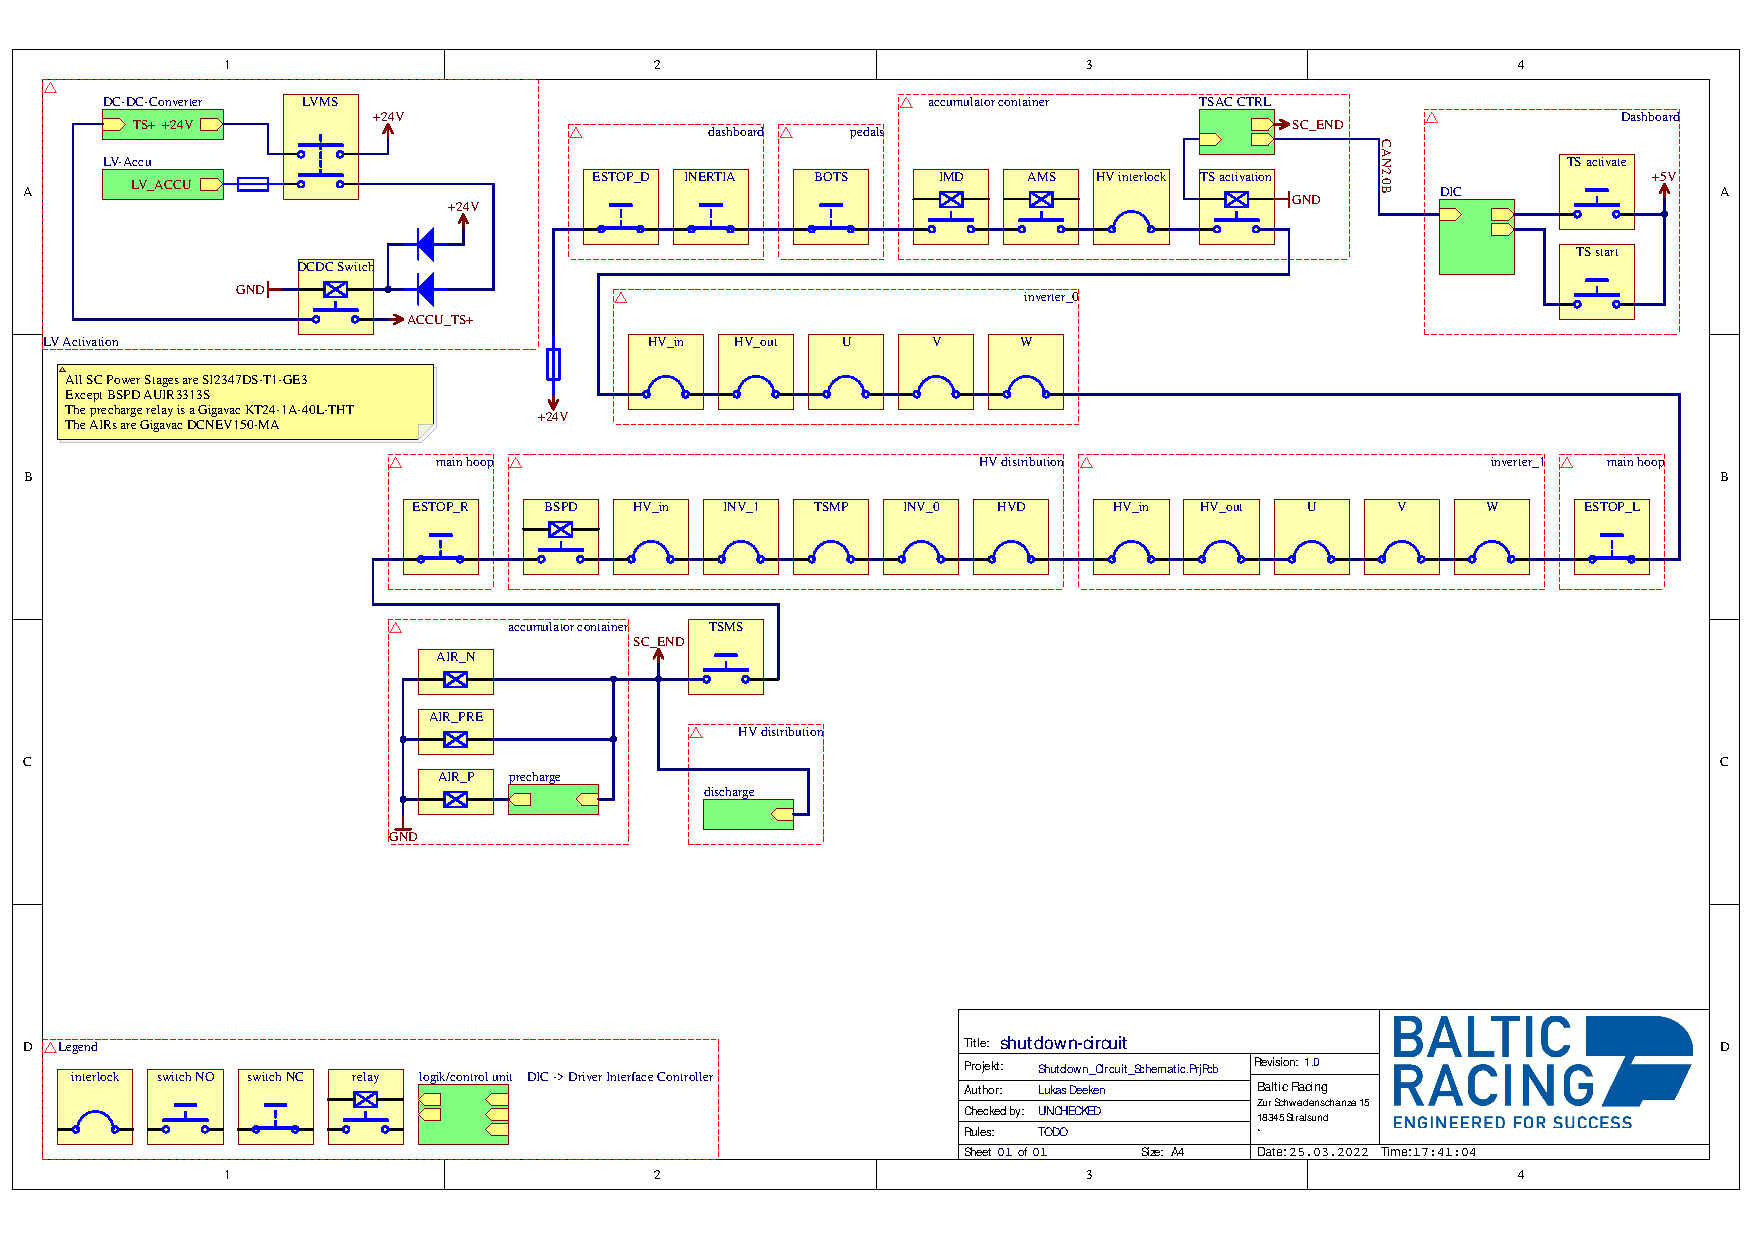
\includegraphics[width=1\linewidth]{bilder/Shutdowncircuit}
	\caption{\ac{SDC} Schaltplan}
	\label{fig:shutdowncircuit}
\end{figure}

In der obenstehenden Graphik ist der sogenannte \ac{SDC} abgebildet. Oben Links befindet sich die Versorgung bzw. der Anfang des \ac{SDC} bestehend aus dem Kickstarter für den \ac{HV}-DCDC und der Hauptschaltung für den \ac{LVMS}. Oben rechts befindet sich die \ac{TS}-aktivierungs-Logik. Im Dashboard des Fahrzeuges befinden sich 2 Knöpfe, einer um das \ac{TS} einzuschalten und einer um die Motoren freizuschalten und damit das Losfahren zu ermöglichen. Die Kommunikation erfolgt hier über den \ac{CAN}-Bus direkt zum \ac{AMS}-Master. Auf dem Rest des Schaltplanes ist von oben nach unten der gesamte \ac{SDC} mit all seinen Elementen abgebildet. Am ende des \ac{SDC} befinden sich die \ac{AIR}`s welche direkt vom \ac{SDC} betrieben werden müssen. Weiterhin wird dort das \ac{SDC}\textsubscript{END}-Signal abgezweigt welches den Ausgangsstatus des \ac{SDC} abzweigt und z.b dem Discharge bereitstellt.\\
\\
Wichtig beim \ac{SDC} zu beachten ist das an möglichst vielen Stellen Stichleitungen eingebracht werden um den \ac{SDC} überwachen zu können. Dies hilft enorm bei der Fehlereingrenzung. Weiter sollte der Querschnitt der Kabel nicht zu dünn gewählt sein. Der Strom im \ac{SDC} liegt bei ca. 0,24 A, da hierüber die \ac{AIR}`s direkt geschaltet werden müssen und hat am ende eine beträchtliche Länge im Fahrzeug und damit einen nicht zu vernachlässigen Widerstand. 
\FloatBarrier
\subsection{Kabeldimensionierung}
%Quelle
Bei Der Kabeldimensionierung wurden 2 unterschiedliche Ansätze angewandt. Einmal die Dimensionierung nach DIN VDE 0298-4 und einmal anhand einer Tabelle. Zweiteres empfiehlt sich standardmäßig für so gut wie alle Anwendungen. Ersterer ist hierbei nur für die Stromführenden \ac{HV}-Leiter sinnvoll anzuwenden. Die Querschnittberechnung ließe sich mit einem physikalischen Modell noch weiter treiben, auf dies wurde jedoch aufgrund des Zeitmangels verzichtet.
Folgend ist einmal die bisher verwendete Tabelle \ref{fig:wire-thickness} aufgeführt. Die Quelle der Tabelle war http://www.learn-about-electronics.com/ allerdings ist dies mittlerweile nicht mehr aufzufinden
Bei der Tabelle ist zu beachten das die Ströme für Chassis Wiring verwendet werden. Unter Power Transmission versteht man hier Leiter die mit geringen Verlusten z.b in einer industriellen Umgebung Ströme über lange Wege z.b. von Haus zu Haus leiten sollen.
\begin{figure}[h]
	\centering
	\includegraphics[width=0.7\linewidth]{"bilder/Wire thickness"}
	\caption{Leiterquerschnitts-Tabelle}
	\label{fig:wire-thickness}
\end{figure}

Nun soll im Anschluss einmal die Berechnung der Querschnitte nach DIN VDE 0298-4 (Anhang) dargestellt werden.\\
Nach 9.4 können wir für ungleichmäßige Ströme den Quadratischen Mittelwert zur Leiterquerschnittbestimmung ansetzen. Den Quadratischen Mittelwert des Stromes der Elektromotoren erhalten wir indem wir das mittlere Drehmoment am Elektromotor bestimmen, hierfür müssen wir auf die Daten aus der \ac{LTS} zurückgreife, in Zukunft empfiehlt es sich die Berechnung einmal mit den Daten aus dem tatsächlichen Fahrzyklus nachzurechnen. Das Drehmoment was wir hier erhalten liegt bei 68,2 Nm pro Motor. Im Handbuch des Emrax 208 (Anhang) befindet sich ein Parameter der uns den \acfirst{RMS}-Strom in A pro NM Drehmoment an der Ausgangswelle angibt. Dieser liegt bei 0,8 Nm/A\textsubscript{RMS}. \\
Damit lässt sich ermitteln das der Quadratische Mittelwert des Stromes bei ca. 85,3 A liegt\\
Nun lässt sich mit Hilfe von Tabelle 9.2 der Strom für den Verlegungstyp E (Verlegung wie Motorleiter) für verschiedene Kabelquerschnitte ermitteln. Wir ermitteln für 16 mm\^2 einen Strom von 80 A für 3 belastete Leiter und für 25 mm\^2 respektive einen Strom von 101 A. Zur Sicherheit wurde hier an der Stelle auf 25 mm\^2 zurückgegriffen, allerdings sollten in Zukunft durchaus mal Versuche mit 16 mm\^2 für die Motorleiter unternommen werden da dies zu einer durchaus signifikanten Gewichtsersparnis führen kann.\\
\\
Für den \ac{DC}-Bus wurde das gleiche vorgehen angewandt. Hier bekommen wir den Strom direkt aus der \ac{LTS} mit 53 A. Das ergibt nach Typ E mit 2 belasteten Leitern 10 mm\^2 Querschnitt. Jedoch konnten wir keine Steckverbinder finden welche 10 mm\^2 Kabel akzeptiert und ein entsprechendes Rating hat weshalb wir hier auf 16 mm\^2 und damit einen max. Strom von 80 A gegangen sind. Auch hier gilt wieder das noch Möglichkeiten der Gewichtsersparnis bestehen.\\

\FloatBarrier
\subsection{Hochvolt Kabelbaum}

\begin{figure}[h]
	\center
	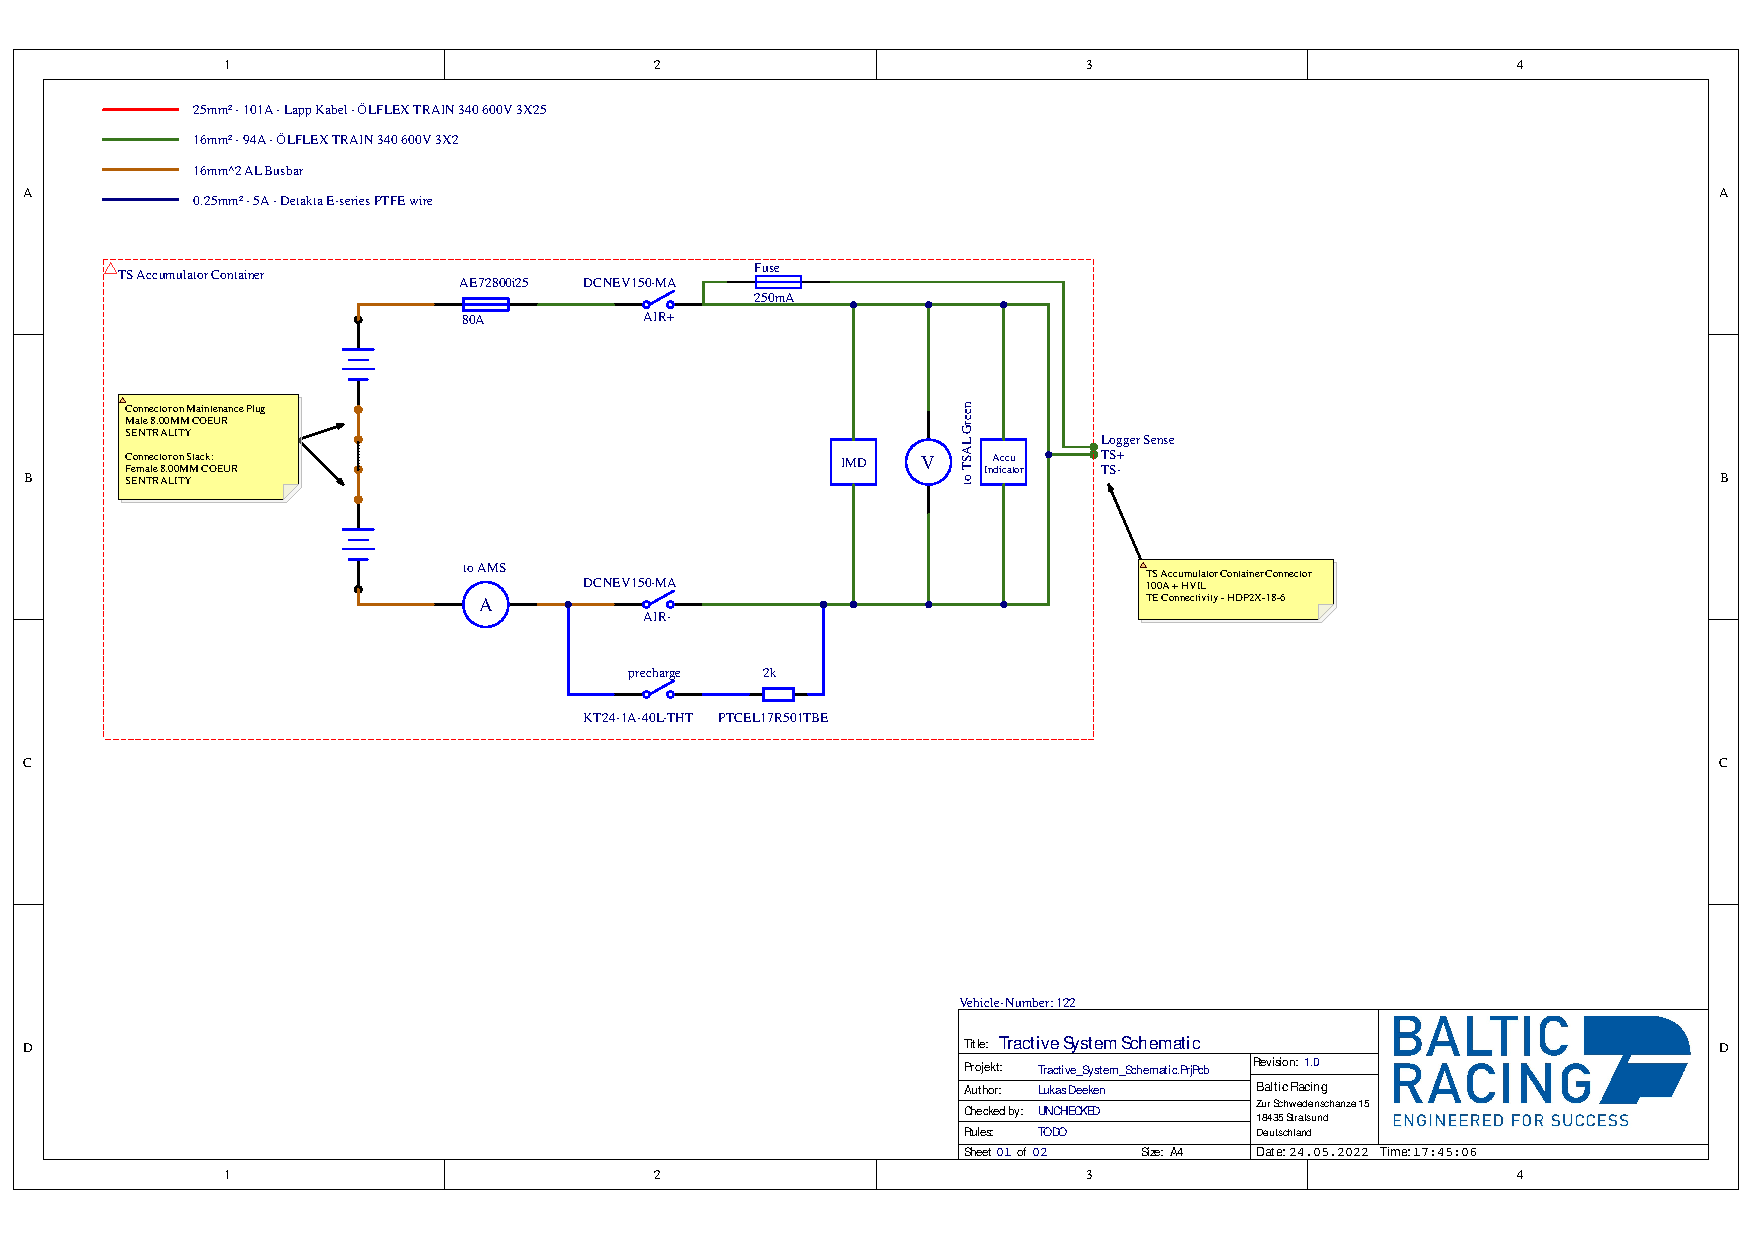
\includegraphics[page=1,width=1\linewidth]{bilder/Tractive_System_Schematic_V4.pdf}
	\caption[\ac{TS} Schaltplan Seite 1]{}
	\label{fig:tractivesystemschematic1}
	
	\center
	\includegraphics[page=2,width=1\linewidth,]{bilder/Tractive_System_Schematic_V4.pdf}
	\caption[\ac{TS} Schaltplan Seite 2]{}
	\label{fig:tractivesystemschematic2}
	\end{figure}

Der HV Kabelbaum besteht aus 3 Kabelsträngen, einer befindet sich innerhalb des Akkus, einer innerhalb der \ac{HV}-Distribution und einer verbindet diese beiden Geräte sowie die Motoren und die Umrichter miteinander.\\
\\
Wichtig zu beachten ist das alle \ac{HV}-Kabel Orange und entsprechend isoliert sein müssen. Außerdem dürfen \ac{HV}- und \ac{LV}/-Kabel nicht zusammen verlegt werden bzw. sollte es der Fall sein müssen die \ac{LV}-Kabel auch nach \ac{HV} Spezifikation isoliert sein.\\
Es gilt besondere Achtsamkeit bei den Leiterquerschnitten sowie den Mindestbiegeradien an den Tag zu legen. Bei den Steckern ist besonders das Spannungsrating Problematisch, da hier gerne nur das \acfirst{AC}- oder \ac{DC}/-Rating gegeben wird und hier dann entsprechend umzurechnen ist. Hierbei wird das \ac{AC}-Rating mal 1,41 gerechnet um das korrespondierende \ac{DC}-Rating zu erhalten. \\
\\
Bei den \ac{HV}-Leitern ist die Möglichkeit von Aluminium Leitern interessant. Hier wurde damals von der Firma Coroflex die Zusage gemacht das sollte ein Auftrag für ein derartiges Kabel reinkommen, würde man für das Team eine entsprechende Menge kostenlos mit fertigen. Evtl. ließe sich hier in Zusammenarbeit mit anderen Teams eine nennenswerte Menge abnehmen so das sich die Produktion für ein Unternehmen lohnt. Hierbei allerdings beachten das die bisherige Dimensionierung nur für Kupferkabel gilt und dementsprechend im besten Fall noch einmal mit dem Unternehmen zusammen durchgeführt werden sollte.\\
\\
Ansonsten gilt zu beachten das man gerade diese Mehradrigen Kabel, sprich Kabel mit 3 mal 25 mm\^2, wie sie dieses Jahr verwendet werden nicht serienmäßig in orangener Ausführung bekommt, was bedeutet, dass man das Kabel auf jeden Fall einmal in orangenen Schrumpfschlauch einschrumpfen muss. In diesem Zuge wurde auch die Schirmung um die Kabel selbst eingebracht da dies im Gegensatz zur kommerziellen Lösung eine Gewichtsersparnis von ca. 1 kg auf das gesamte Fahrzeug brachte. Außerdem sollten jegliche Stellen wo die Isolierung der \ac{HV}-Kabel verletz wird z.b an Kabelschuhen etc. immer ein Schrumpfschlauch mit Innenkleber angebracht werden. Es empfehlen sich besonders Schläuche mit einem Schrumpfungsverhältnis 3:1. Hierbei gilt zu beachten das es diese Schläuche \ac{idR} auch nicht in Orange gibt weshalb in dem Fall immer ein Klebeschrumpfschlauch als auch ein orangener angebracht werden sollte. Für die mehradrigen Kabel wurde sich entschieden da diese insgesamt eine Gewichtsersparnis bringen und am Ende für ein deutlich saubereres und ordentlicheres Gesamtbild sorgen. Bei der Montage der \ac{HV}-Leiter ist zu beachten das alle Verbindungen bei der Montage wie z.b. die Verschraubung der Kabelschuhe an die \ac{TSMP} fotografiert werden bevor sie in Schrumpfschlauch etc. eingepackt werden. Dies ist für die technische Abnahme notwendig, damit der Prüfer die saubere Montage der Verbindung überprüfen kann, ohne das etwaiger Schrumpfschlauch wieder entfernt werden muss. Weiterhin hat Isoband im Bereich \ac{HV} absolut keine sichere Wirkung und wird auch von der \ac{FSG} nicht als adäquater Isolator angesehen. Für alle Verbindungen etc. gilt stets diese nach Datenblatt zu machen. Heißt wenn beim \ac{TSMP}-Steckverbinder eine schraube und eine Mutter dabei sind dann werden diese verwendet und nicht Mechanismen zur Schraubensicherung erdacht. Weiterhin gilt zu beachten das jeder einzelne stromführende Leiter einzeln abgesichert sein muss. Dies erschwert z.b das parallel schalten von mehreren Pins in einem Steckverbinder zum leiten des Stromes da dann am Steckverbinder für jeden parallelen Kontakt entsprechende Sicherungen vorgesehen sein müssen. Dem aufmerksamen Leser fällt an dieser Stelle auf das bei dem Elektromotor in allen drei Leitern keine separaten Sicherungen vorgesehen sind. Dies lässt sich darauf zurückführen das der Umrichter zugekauft ist und laut Datenblatt über einen entsprechenden Überstromschutz verfügt. Im Selbstbau Fall müssten hier 3 Sicherungen wie aus dem Akku bekannt verbaut werden. 
 
 \FloatBarrier
\subsection{Sicherungsauslegung}
Die Sicherung muss stets der schwächste Teil eines Stromkreises sein. In diesem Sinne muss also bei der Auslegung der Stecker darauf geachtet werden das deren Rating höher ist als das der Sicherung oder wir müssen im Umkehrschluss schauen dass, das Rating der Sicherung niedriger ist als das der anderen Komponenten. Für \ac{DC}-Sicherungen mit einer derart hohen Betriebsspannung und einem derart hohen Kurzschlussstrom reichen Flachstecksicherung wie sie im \ac{LV}-Bereich zu finden sind nicht mehr aus. Hier müssen z.b sandgefüllte Sicherungen verwendet werden. Sinn dahinter ist es den Lichtbogen der sich beim durchbrennen der Sicherung bildet zu löschen. Dies ist bei einer typischen \ac{LV}-Sicherung nicht gegeben. Zum Thema Kurschlussrom, dieser errechnet sich aus dem Innenwiederstand des gesamten Akkus und der anliegenden Spannung. Wir Rechnen hier immer im schlimmsten Fall sprich alle Zellen sind was den Innenwiederstand angeht eher im niedrigeren Bereich und der Akku ist voll geladen. Dabei reden wir von 556,75 V Spannung und 0,528 $\Omega$ Innenwiederstand !!!!(Berechnung des Innenwiederstands einfügen 132S 5P 0,02Ohm pro zelle)!!!! Daraus ergibt sich ein Kurzschlussstrom von 1054 A. Der Kurzschlussstrom sollte mit dem rated breaking current verglichen werden. Ist der Kurzschlussstrom niedriger ist die Sicherung geeignet. Dann haben wir bei der Sicherung das Spannungsrating welches eingehalten werden muss. Auf Basis dieser Daten kann eine Sicherung bzw. eine Baureihe herausgesucht werden. In unserem Fall ergaben die Recherchen die AE7 EV Fuse von Adler Elektrik. Die Querschnittberechnung hat ein Kabel von 16 mm\^2 und daher 80 A ergeben. Diese 80 A legen wir auch bei der Sicherung zu Grunde. Dies ergibt die AE72800i25. Daraufhin lässt sich im Datenblatt am Zeit-Strom Schaubild \ref{fig:zeitstromtsfuse} ablesen wie lange die Sicherung bei Unterschiedlichen Strömen braucht um auszulösen. Es ergibt sich eine zeit von ca. 400 s bei einem Strom von 150 A und eine Zeit von ca. 0,5 ms bei Kurzschlussstrom.

\begin{figure}[h]
	\centering
	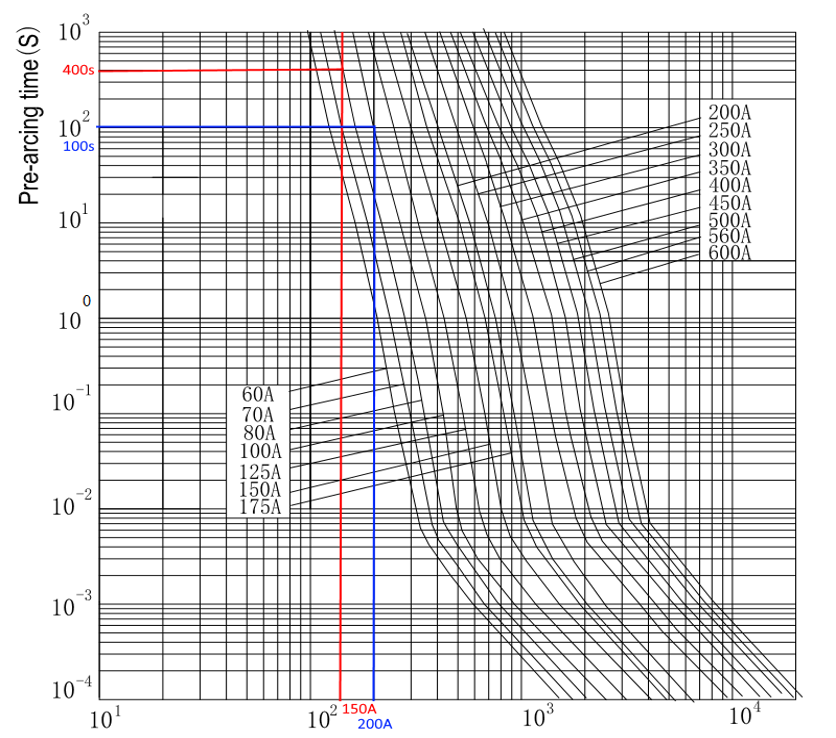
\includegraphics[width=0.7\linewidth]{bilder/Zeit_Strom_TSFUSE}
	\caption{}
	\label{fig:zeitstromtsfuse}
\end{figure}

\FloatBarrier
\subsection{Steckverbinder Auswahl}
Parameter für die Steckverbinder Auswahl sind analog zur Kabelauswahl, die Betriebsspannung als auch der Betriebsstrom. Die Auswahl der Steckverbinder erfolgt im Zuge des Systemdesigns wo die Schnittstellen und die Anforderungen an diese festgelegt wurden. Der gewählte Steckverbinder sollte über ausreichend Plätze in der richtigen Stärke verfügen um den Anforderungen gerecht zu werden. Hierbei ist interessant welche Pins man für die Steckplätze bekommen kann. Oft ist es so möglich durch unterschiedlich große Steckplätze die gleichen Kabelquerschnitte zu bekommen. Da es selten Steckverbinder gibt die genau zu dem vorliegenden System passen kann dies sehr nützlich sein um das einsetzten eines deutlich größeren und damit schwereren als auch teureren Steckverbinders zu verhindern. Auch bei den Pins gilt es stets die Stromratings zu beachten. Bei gerade solchen Kabel zu Kabel Verbindern die dazu dienen Kabel in ein Gehäuse zu führen ist es sinnvoll ein paar Steckplätze im Design frei zu lassen um es zu ermöglichen im Nachhinein einfach weitere Kabel hinzuzufügen, sollte dies später einmal notwendig werden. Auch führt dies dazu dass bei Änderung am Systemdesign die Interfaces der Geräte potentiell gleich bleiben können, was den Test und Aufbauprozess des Fahrzeuges vereinfacht. 
Bei der Auswahl der Steckverbinder ist immer drauf zu achten das entsprechende Crimp- als auch Auspinn- bzw. Einpinn/-Werkzeuge mit beschafft werden damit die Montage der Verbinder anschließend auch reibungsfrei klappt. Weiter ist auf zusätzliches Kabelzubehör wie Endkappen, Blindstecker, Staubschutzkappen usw. zu achten bzw. mit zu beschaffen. Außerdem ist es üblich die Gehäuse der Steckverbinder und die Pins separat zu bestellen sodass auch hierauf geachtet werden muss. Gerade bei der Beschaffung der Pins empfiehlt es sich mindestens um den Faktor 1,5 mehr zu bestellen als benötigt da hier öfter Ausschuss produziert wird. Auch die Steckverbinder können beim Ein- bzw. Aus/-pinnen kaputt gehen so das man hiervon Ersatz vorhalten sollte.\\
Eine Besonderheit bei den \ac{HV}-Steckern stellt die Interlockleitung dar. Ziel dieser Leitung ist es das \ac{HV}-System abzuschalten sobald ein Steckverbinder gezogen wird um einen elektrischen Schlag durch berühren der Kontakte im Steckverbinder zu verhindern. Hierbei handelt es sich meist um ein oder zwei weitere Steckkontakte im \ac{HV}-Stecker wo Kabel mit deutlich geringerem Querschnitt angeschlossen werden können. Wichtig hierbei ist das diese Interlockleitung aufgehen muss bevor eine vollständige Trennung des Steckverbinder erfolgt. 

\FloatBarrier
\subsection{\acfirst{HVD}}
Der \ac{HVD} befindet sich mittig am Heck des Fahrzeuges. Sinn dieses Steckverbinders ist es eine mechanische und damit elektrische Öffnung des \ac{HV}-Systems zwischen Akku und Umrichter zu ermöglichen. Dies kann notwendig werden wenn z.b. die \ac{AIR}`s den Dienst verweigern und damit eine Möglichkeit der Trennung der Motoren vom Betriebsstrom anderweitig nicht mehr möglich machen. Bei diesem Steckverbinder kann es sich entweder um dafür vorgesehene Service Trennschalter aus einem regulären Elektrofahrzeug handeln oder um modifizierte Steckverbinder welche auch für den Akku verwendet werden. Die modifizierten sind dabei in der Regel kleiner, leichter und günstiger.

\FloatBarrier
\subsection{\ac{AIR}}
Datenblatt werte, worauf muss ich achten
Break Open Current

Zeichnung zu diesem relai typ

Die \ac{AIR}`s haben es zum ziel das \ac{HV}-Netz des Akku galvanisch vom restlichen Fahrzeug zu trennen indem mit einem Relais \ac{HV}+ und mit dem anderen Relais \ac{HV}- geöffnet wird. Bei diesen Relais handelt es sich in der Regel um, \acfirst{SPST} \acfirst{NO} Relais mit \acfirst{AUX} Kontakten. Heißt wir haben einen Steuerkreis und einen Lastkreis. Im stromlosen Zustand ist der Lastkreis geöffnet und wir haben einen vom Lastkreis getrennten Kreis welcher synchron zum Lastkreis geschaltet wird und somit eine Überwachung des Schaltzustandes des Lastkreises ermöglicht.\\
Bei der Auswahl des Relais ist auf das Spannungsrating als auch das Stromrating zu achten, aber auch auf die Schaltspannung, sprich die Spannung des Steuerkreises. Weiter ist der Schaltstrom ein interessantes Kriterium, da es sich bei solch einer Relaisspule um eine Induktive Last handelt liegt ein recht hoher Einschaltstrom vor, welcher vom speisenden Netz getragen werden können muss, in unserem vom \ac{SDC}. Für den TY22 wurde das DCNEV150-M von Littlefuse gewählt.

\FloatBarrier
\section{Ladesystem / Handcart}

Das Handcart dient einerseits zum Transport des Akku außerhalb des Fahrzeuges als auch zum laden des Akku. Die Auswahl des Ladegerätes beschränkte sich an der Stelle auf ein Gerät welches wir von der Firma Schulz Elektronik kostenlos bekommen konnten. Hierbei ist dennoch zu beachten das dieses gerät die Ladeschlussspannung erreichen kann sprich 600+ Volt abbilden können sollte, als auch über ein programmierbares Steuerinterface verfügen sollte, so das eine automatisierte Laderegelung ermöglicht wird. Weiter ist die Leistung des Gerätes interessant, mehr ist hierbei erst einmal besser, wobei 15 KW mehr als ausreichen sollten da hiermit ein 7,5 KWh Akku in ca. 30 min geladen werden kann.\\
Beim dem Design des Handcartes ist sowohl in elektrischer- als auch mechanischer/-Hinsicht auf Regelkonformität zu achten. Einerseits gibt es Reglementierung für die maximalen mechanischen Abmaße als auch der Einsatz einer Totmannbremse. andererseits muss das Handcart wie das Fahrzeug über \ac{TSMP}, \ac{IMD}-Licht uvm. verfügen. Besondere Anforderung ist hierbei das beim laden der Status des Akku ausgegeben werden können muss. Heißt die Spannung als auch die Temperatur der Zellen muss Anzeigbar sein. Dies ist beim TY22 über eine \acfirst{USB}-Verbindung von einem Raspberry Pi zum \ac{AMS} geplant. Der Raspberry Pi ist dabei mit einem Touchdisplay ausgestattet und ermöglicht so die Ausgabe der \ac{AMS}-Daten als auch die Steuerung des Ladevorganges. Zu guter Letzt ist zu beachten dass, das Ladegerät mit in den \ac{SDC} eingebunden werden muss. Dies erfolgt beim Handcart für den TY22 über einen abgriff des \ac{SDC}\textsubscript{END} Signales und eine hierüber erfolgende Ansteuerung eines Relais welche die Interlockleitung des Ladegerätes öffnet oder trennt. Ein trennen dieser Leitung führt laut Datenblatt zu einem unmittelbaren herunterfahren des Ladegerätes.

\begin{figure}
	\centering
	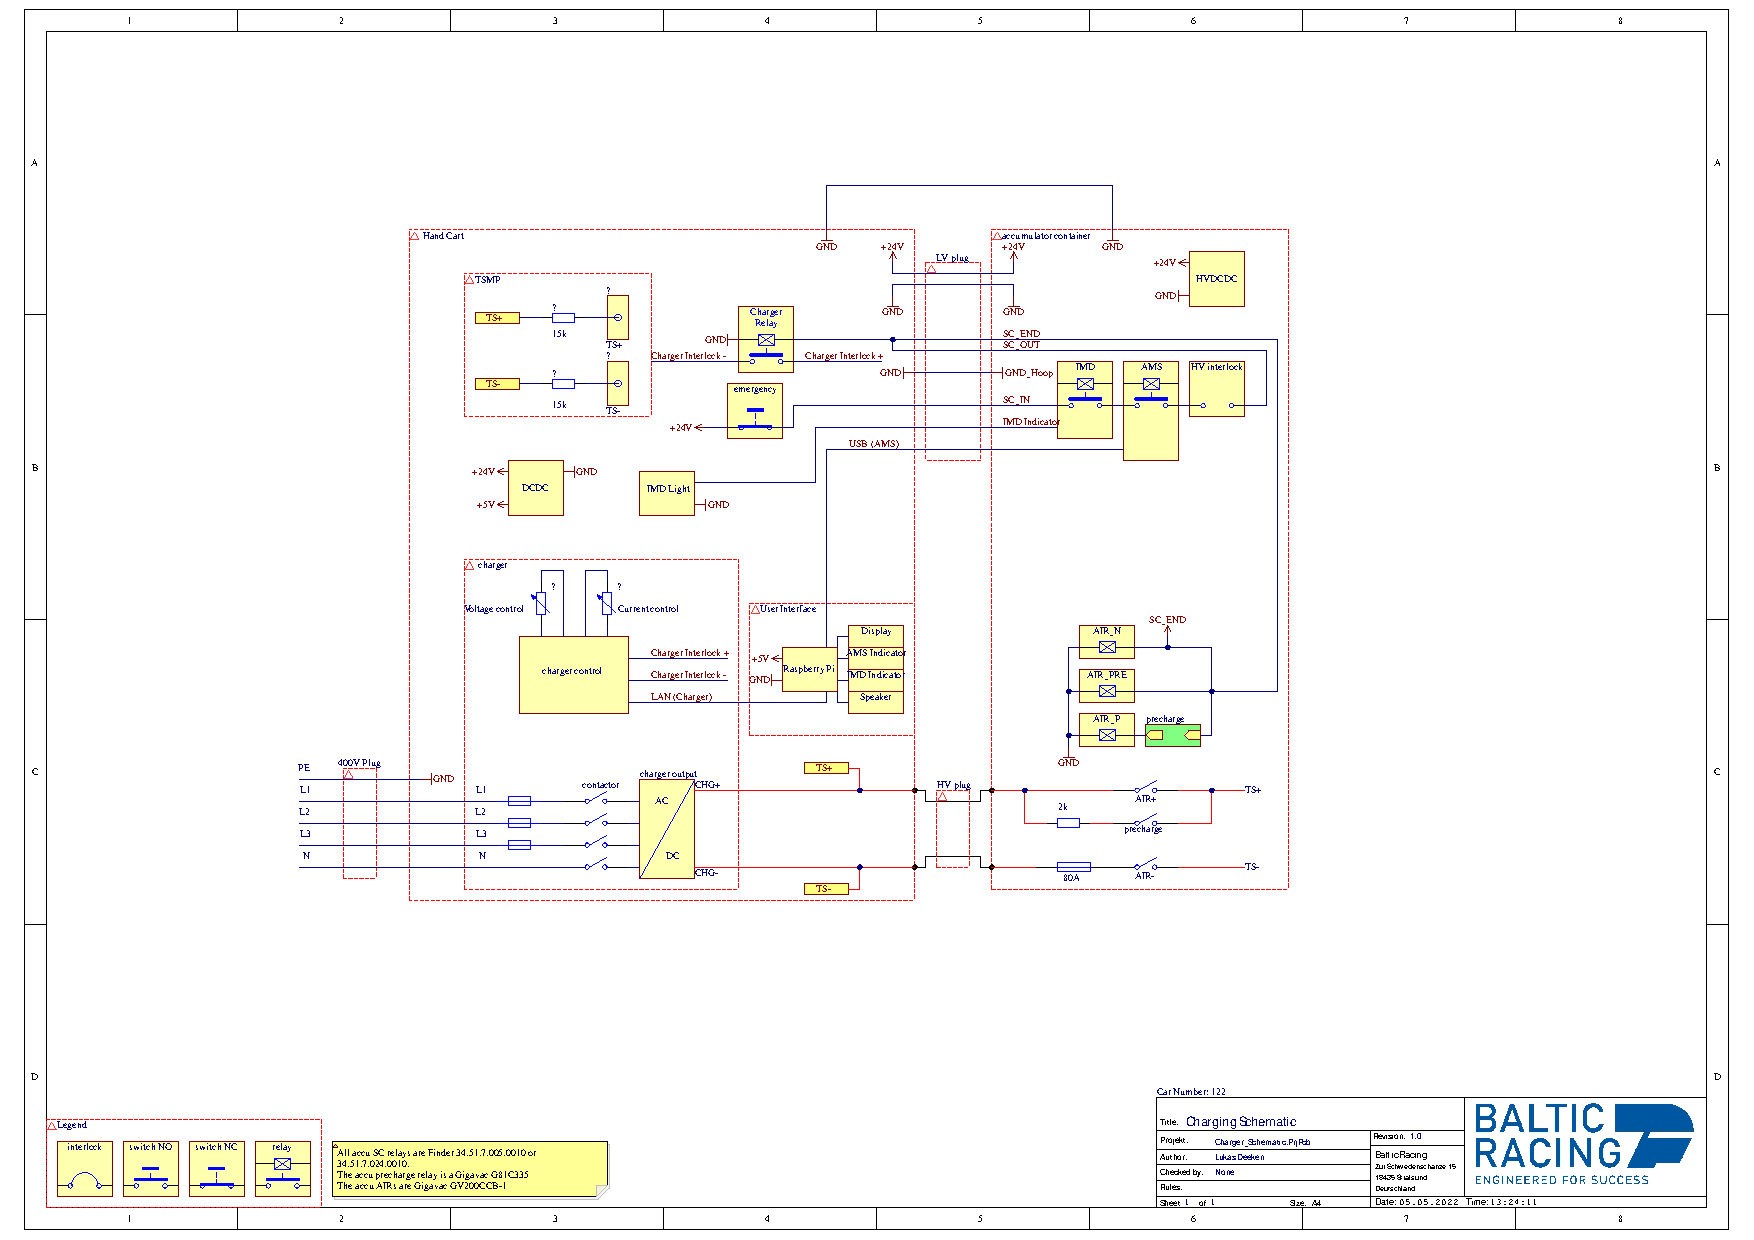
\includegraphics[width=1\linewidth]{C:/Users/lukas/Desktop/Charger_Schematic_V3}
	\caption{Schaltplan Handcart}
	\label{fig:chargerschematicv3}
\end{figure}

\FloatBarrier
